%%%%%%%%%%%%%%%%%%%%%%%%%%%%%%%%%%%%%%%%%%%%%%%%%%%%%%%%%%%%%%%%%%%%%%%%
% mimir.tex
%
% This document describes the \Mimir\ indexing and search framework.
%
% $Id$
%%%%%%%%%%%%%%%%%%%%%%%%%%%%%%%%%%%%%%%%%%%%%%%%%%%%%%%%%%%%%%%%%%%%%%%%


%%%%%%%%%%%%%%%%%%%%%%%%%%%%%%%%%%%%%%%%%%%%%%%%%%%%%%%%%%%%%%%%%%%%%%%%
\documentclass[10pt, a4paper, twoside]{report}
%%%%%%%%%%%%%%%%%%%%%%%%%%%%%%%%%%%%%%%%%%%%%%%%%%%%%%%%%%%%%%%%%%%%%%%%%%%%
%
% Valentin Tablan 13/02/2002
%
% $Id: preamble.tex,v 1.8 2004/07/14 13:51:44 valyt Exp $
%
% This file is designed to be included at the begining of any latex document 
% and handles things like pdf detection, tex4ht detection, notes command, 
% paragraph spacing and indenting.
%
% 28/July/2003: consolidated GATE utils and TAO main.tex stuff here (Hamish).
%
%%%%%%%%%%%%%%%%%%%%%%%%%%%%%%%%%%%%%%%%%%%%%%%%%%%%%%%%%%%%%%%%%%%%%%%%%%%%


%%%%%%%%%%%%%%%%%%%%%%%%%%%%%%%%%%%%%%%%%%%%%%%%%%%%%%%%%%%%%%%%%%%%%%%%%%%%
% PDF detection
%%%%%%%%%%%%%%%%%%%%%%%%%%%%%%%%%%%%%%%%%%%%%%%%%%%%%%%%%%%%%%%%%%%%%%%%%%%%

\usepackage{ifpdf}

%%%%%%%%%%%%%%%%%%%%%%%%%%%%%%%%%%%%%%%%%%%%%%%%%%%%%%%%%%%%%%%%%%%%%%%%%%%%
% tex4ht detection
%%%%%%%%%%%%%%%%%%%%%%%%%%%%%%%%%%%%%%%%%%%%%%%%%%%%%%%%%%%%%%%%%%%%%%%%%%%%

\newif\ifhtml
\ifx\ifHtml\undefined
  \htmlfalse          % we are not running tex4ht
\else
  \htmltrue           % we are running tex4ht
\fi


%%%%%%%%%%%%%%%%%%%%%%%%%%%%%%%%%%%%%%%%%%%%%%%%%%%%%%%%%%%%%%%%%%%%%%%%%%%%
% packages
%%%%%%%%%%%%%%%%%%%%%%%%%%%%%%%%%%%%%%%%%%%%%%%%%%%%%%%%%%%%%%%%%%%%%%%%%%%%

% note that hyperref modifies many of the latex commands so it needs to be 
% the last loaded package.

% general packages
\usepackage[english]{babel}
\usepackage{lscape}
\usepackage{longtable}
\usepackage{setspace}
\usepackage{color}
\usepackage{fancyhdr}
\usepackage{listings}
\usepackage{longtable}
\usepackage{txfonts}
\usepackage[text={5in,8.5in}, hmarginratio=1:1, vmarginratio=1:1]{geometry}
% packages with mode detection 
\ifpdf
  %PDF specific stuff
  \usepackage[pdftex]{graphicx}
  % prefer .pdf graphics if available
  \DeclareGraphicsExtensions{.pdf,.png}
  \usepackage{thumbpdf}

  % this should be last!
  \usepackage[
    pdftex,
    pdfborder=0,
    pdftitle={},
    pdfauthor={},
    pdfsubject={},
    pdfkeywords={},
    pdfpagemode=None,
    colorlinks=false,
    urlcolor=blue,
    anchorcolor=blue,
    anchorcolor=blue,
    filecolor=blue,
    linkcolor=blue,
    citecolor=blue,
    ]{hyperref}
\else
  \ifhtml
    % tex4ht specific stuff
    \usepackage{graphicx}
    \usepackage[colorlinks=false]{hyperref}
    % force .png extension on includegraphics
    \DeclareGraphicsExtensions{.png}
  \else
    % Latex specific stuff
    \usepackage[dvips]{graphicx}

    % this should be last!
    \usepackage[hypertex, colorlinks=false]{hyperref}
  \fi
\fi

%%%%%%%%%%%%%%%%%%%%%%%%%%%%%%%%%%%%%%%%%%%%%%%%%%%%%%%%%%%%%%%%%%%%%%%%%%%%
% HTML support commands
%%%%%%%%%%%%%%%%%%%%%%%%%%%%%%%%%%%%%%%%%%%%%%%%%%%%%%%%%%%%%%%%%%%%%%%%%%%%
% some utility definitions of HTML commands using the hyperref package 
% \htlink{target URL}{link text} - hypertext link
\newcommand{\htlink}[2]{\href{#1}{#2}}
\newcommand{\htlinkplain}[1]{\href{#1}{#1}}

% latex commands that only appear in the HTML version
\newcommand{\htlinkhtml}[2]{\href{#1}{#2}}
\newcommand{\htlinkplainhtml}[1]{\href{#1}{#1}}
\newcommand{\htlatexhtml}[1]{#1}

% \htcode{code} - raw HTML code
\newcommand{\htcode}[1]{}

% \htlatex{code} - latex only code
\newcommand{\htlatex}[1]{#1}

% if we're tex4ht'ing, redefine the HTML commands to use tex4ht commands
\ifhtml
  \renewcommand{\htcode}[1]{\HCode{#1}}
  \renewcommand{\htlatex}[1]{}
\else
  \renewcommand{\htlinkhtml}[2]{}
  \renewcommand{\htlinkplainhtml}[1]{}
  \renewcommand{\htlatexhtml}[1]{}
\fi


%%%%%%%%%%%%%%%%%%%%%%%%%%%%%%%%%%%%%%%%%%%%%%%%%%%%%%%%%%%%%%%%%%%%%%%%%%%%
% notes commands 
%%%%%%%%%%%%%%%%%%%%%%%%%%%%%%%%%%%%%%%%%%%%%%%%%%%%%%%%%%%%%%%%%%%%%%%%%%%%

% writes a small "note:" marker on the left margin of the note 
\newcommand{\notes}[1]
{
\setlength{\unitlength}{1mm}
\begin{picture}(0,0)(15, 0)
\put(0,0) {\framebox{{\scriptsize {\sf {\bf note:}}}}}
\end{picture}%
{\sf{#1}}
\begin{picture}(0,0)
\put(0,0){\rule{.5\baselineskip}{.5\baselineskip}}
\end{picture}%
}

% uncomment for final version.
%%% \renewcommand{\notes}[1]{}

% IF pdf mode is enabled it will create a PDF note (non printable)
\newcommand{\pdfnote}[1]{
  \ifpdf
    \pdfannot         % generic annotation
                      
      width 10cm      % the dimension of the annotation can be controlled
      height 0cm      % via <rule spec>; if some of dimensions in
      depth  4cm      % <rule spec> is not given, the corresponding
                      % value of the parent box will be used.
    {                 
      /Subtype /Text  % text annotation
      %/Open true     % if given the text annotation opened by default
      /Contents       % text contents
        (#1)
    }
  \else
  \notes{#1}
  \fi
}


%%%%%%%%%%%%%%%%%%%%%%%%%%%%%%%%%%%%%%%%%%%%%%%%%%%%%%%%%%%%%%%%%%%%%%%%%%%%
% switches 
%%%%%%%%%%%%%%%%%%%%%%%%%%%%%%%%%%%%%%%%%%%%%%%%%%%%%%%%%%%%%%%%%%%%%%%%%%%%

\textwidth 5in
\textheight 8.5in

%\oddsidemargin 0.1in
%\evensidemargin 0.1in
%\topskip 0.35in
%\footskip 0.2in
%\topmargin -1.1cm
\tolerance=6000

% paragraph break with no indent
\setlength{\parindent}{0pt}

% extra spacing between paragraphs
\setlength{\parskip}{2ex}
%\setlength{\parskip}{1ex plus 0.5ex minus 0.2ex}

% number subsubsections in the TOC
\setcounter{tocdepth}{3}

% spacing
\singlespacing
%\onehalfspacing
%\doublespacing



%%%%%%%%%%%%%%%%%%%%%%%%%%%%%%%%%%%%%%%%%%%%%%%%%%%%%%%%%%%%%%%%%%%%%%%%%%%%
% misc commands 
%%%%%%%%%%%%%%%%%%%%%%%%%%%%%%%%%%%%%%%%%%%%%%%%%%%%%%%%%%%%%%%%%%%%%%%%%%%%

\newcommand{\delete}[1]{}
\newcommand{\omitted}[1]{{\small \sf =OMITTED=}}
\newcommand{\thing}{book}

\definecolor{cmdcol}{RGB}{0, 0, 128}
\newcommand{\cmd}[1]{\textcolor{cmdcol}{\textbf{\texttt{#1}}}}

%%%%%%%%%%%%%%%%%%%%%%%%%%%%%%%%%%%%%%%%%%%%%%%%%%%%%%%%%%%%%%%%%%%%%%%%%%%%
% sectioning commands 
%%%%%%%%%%%%%%%%%%%%%%%%%%%%%%%%%%%%%%%%%%%%%%%%%%%%%%%%%%%%%%%%%%%%%%%%%%%%

\newcommand{\chapt}[1]{\section{#1}}
\newcommand{\sect}[1]{\subsection{#1}}
\newcommand{\subsect}[1]{\subsubsection{#1}}
\newcommand{\subsubsect}[1]{{\bf #1}}
\newcommand{\subsubsubsect}[1]{{\bf #1}}
\newcommand{\chapthing}{section}
\newcommand{\Chapthing}{Section}
\newcommand{\chapthings}{sections}
\newcommand{\Chapthings}{Sections}

\renewcommand{\chapt}[1]{\chapter{#1}}
\renewcommand{\sect}[1]{\section{#1}}
\renewcommand{\subsect}[1]{\subsection{#1}}
\renewcommand{\subsubsect}[1]{\subsubsection{#1}}

\renewcommand{\chapthing}{chapter}
\renewcommand{\Chapthing}{Chapter}
\renewcommand{\chapthings}{chapters}
\renewcommand{\Chapthings}{Chapters}


%%%%%%%%%%%%%%%%%%%%%%%%%%%%%%%%%%%%%%%%%%%%%%%%%%%%%%%%%%%%%%%%%%%%%%%%%%%%
% compact itemize etc. 
%%%%%%%%%%%%%%%%%%%%%%%%%%%%%%%%%%%%%%%%%%%%%%%%%%%%%%%%%%%%%%%%%%%%%%%%%%%%

% store the current value of parskip and allow resetting
% via \resetparskip
\newlength{\oldparskip}
\setlength{\oldparskip}{\parskip} 
\oldparskip=\parskip 
\newcommand{\resetparskip}[0]
{
  \parskip=\oldparskip
}

% \bit, \eit - compact version of itemize
% note that parskip is changed. To reset it use \resetparskip
% (after any text following the list that's not a new paragraph)
\newcommand{\bit}[0]
{
  \parskip=-4pt
  \begin{itemize}
  \itemsep=-3pt
}
\newcommand{\eit}[0]
{
  \end{itemize}
  \resetparskip
}

% \ben, \een - compact version of enumerate
% note that parskip is changed. To reset it use \resetparskip
% (after any text following the list that's not a new paragraph)
\newcommand{\ben}[0]
{
  \parskip=-4pt
  \begin{enumerate}
  \itemsep=-3pt
}
\newcommand{\een}[0]
{
  \end{enumerate}
  \resetparskip
}

% \bde, \ede - compact version of description
% note that parskip is changed. To reset it use \resetparskip
% (after any text following the list that's not a new paragraph)
\newcommand{\bde}[0]
{
  \parskip=-4pt
  \begin{description}
  \itemsep=-3pt
}
\newcommand{\ede}[0]
{
  \end{description}
  \resetparskip
}


%%%%%%%%%%%%%%%%%%%%%%%%%%%%%%%%%%%%%%%%%%%%%%%%%%%%%%%%%%%%%%%%%%%%%%%%%%%%
% font size
%%%%%%%%%%%%%%%%%%%%%%%%%%%%%%%%%%%%%%%%%%%%%%%%%%%%%%%%%%%%%%%%%%%%%%%%%%%%

% font size - uncomment for standard print
\newcommand{\nsmall}{\small}
\newcommand{\nnormalsize}{\normalsize}
\newcommand{\nlarge}{\large}

% font size - uncomment for large print
%\newcommand{\nsmall}{\normalsize}
%\newcommand{\nnormalsize}{\Large}
%\newcommand{\nlarge}{\Large}


%%%%%%%%%%%%%%%%%%%%%%%%%%%%%%%%%%%%%%%%%%%%%%%%%%%%%%%%%%%%%%%%%%%%%%%%%%%%
% quotex - including quotes in documents
%%%%%%%%%%%%%%%%%%%%%%%%%%%%%%%%%%%%%%%%%%%%%%%%%%%%%%%%%%%%%%%%%%%%%%%%%%%%

% create the .qt aux file
\newcommand{\qtinit}{
  \newwrite\qtaux
  \immediate\openout\qtaux=\jobname.qta
  \immediate\write\qtaux{! \jobname.qta}
}

% record the name of a quotable file
\newcommand{\qtpath}[1]{
  \immediate\write\qtaux{qtpath: #1}
}

% include a quote
\newcommand{\qt}[1]{
  \newread\qtfile
  \immediate\openin\qtfile=qt_#1.tex
  \ifeof\qtfile
    \immediate\closein\qtfile
    \immediate\write\qtaux{quote: #1}
  \else
    \immediate\closein\qtfile
    \input{qt_#1}
  \fi
}

% commands re-defined by the quotes files
\newcommand{\qtauthor}{}
\newcommand{\qttitle}{}
\newcommand{\qtdate}{}
\newcommand{\qtquote}{}
\newcommand{\qtpage}{}
\newcommand{\qtall}{}


%%%%%%%%%%%%%%%%%%%%%%%%%%%%%%%%%%%%%%%%%%%%%%%%%%%%%%%%%%%%%%%%%%%%%%%%%%%%
%%%%%%%%%%% Support for including code listings %%%%%%%%%%%%%%%%%%%%%%%%%%%%
%%%%%%%%%%%%%%%%%%%%%%%%%%%%%%%%%%%%%%%%%%%%%%%%%%%%%%%%%%%%%%%%%%%%%%%%%%%%

% Generic settings

\lstset{
  language=Java,
  keywordstyle=\color{blue}\bfseries,
  commentstyle=\color[rgb]{0,0.5,0}\it,
  stringstyle=\color[rgb]{1,0,1},
  showstringspaces=false,
  rulesepcolor=\color[rgb]{0.8,0.8,0.8},
  captionpos=b
}

% Normal size for listings
\newcommand{\lstnormal}{
\lstset{
  basicstyle=\footnotesize\ttfamily,
  numbers=left, 
  numberstyle=\tiny,
  stepnumber=1,
  numbersep=10pt,
  xleftmargin=20pt,
  frame=shadowbox,
  frameround=ffff,
  framesep=6pt,
  framexleftmargin=5mm
}
}

% Define a compact listings mode
\newcommand{\lstcompact}{
\lstset{
  basicstyle=\scriptsize\ttfamily,
  numbers=none, 
  xleftmargin=0pt,
  frame=none,
  breaklines=true
}
}

% by default, we start with the normal size
\lstnormal
 

\newcommand{\Mimir}{M\'{i}mir}
\begin{document}

\begin{titlepage}
\thispagestyle{empty}

\setlength{\unitlength}{1mm}
\begin{picture}(150, 0)
\color{mimirblue}
\linethickness{10mm}
\put(0, 3){\line(1,0){125}}
\put(1, 0){\textcolor{white}{\Huge \textsc{\textbf{\Mimir}}}}
\end{picture}

{\Large \sc Multi-paradigm Information Management\\Index and Repository}

\vspace{30mm}
{\Huge \textsc{A User Guide}}


\vspace{30mm}
{\Large Valentin Tablan \hspace{1cm} Ian Roberts}

\vspace{5mm}
{\bf \today}\\
{\bf version 4.0-SNAPSHOT}

\vspace\fill
\begin{picture}(150, 0)
\color{mimirblue}
\linethickness{10mm}
\put(0, 3){\line(1,0){125}}
\end{picture}
\end{titlepage}



\clearpage

\setcounter{tocdepth}{2}
\tableofcontents

\thispagestyle{empty}
\cleardoublepage

\pagestyle{fancy}
\fancyhead{} %clear all headings
\fancyhead[RO,LE]{\Mimir}
\fancyhead[LO, RE]{User Guide}

%%%%%%%%%%%%%%%%%%%%%%%%%%%%%%%%%%%%%%%%%%%%%%%%%%%%%%%%%%%%%%%%%%%%%%%%
% main %%%%%%%%%%%%%%%%%%%%%%%%%%%%%%%%%%%%%%%%%%%%%%%%%%%%%%%%%%%%%%%%%
%%%%%%%%%%%%%%%%%%%%%%%%%%%%%%%%%%%%%%%%%%%%%%%%%%%%%%%%%%%%%%%%%%%%%%%%
\chapter{Introduction}\label{sec:intro}
\Mimir\ is a multi-paradigm information management index and repository which
can be used to index and search over text, annotations, semantic schemas
(ontologies), and semantic meta-data (instance data). It allows queries that
arbitrarily mix full-text, structural, linguistic and semantic queries and that
can scale to gigabytes of text.

A typical semantic annotation project deals with large quantities of data of
different kinds. \Mimir\ provides a framework for implementing indexing and
search functionality across all these data types, listed below in the order of
increasing information density:

{\bf Text}\\
All documents have a textual content. Support for full text search represents
the most basic indexing functionality and it is required in most (if not all)
cases.  Even when semantic annotation is used to abstract away from the
actual textual data, the original content still needs to be accessible so
that it can be used to provide textual query fragments in the case of more
complex conceptual queries.

\Mimir\ uses inverted indexes\footnote{{\em Inverted Indexes} are data
structures traditionally used in Information Retrieval to support indexing of
text.} for indexing the document content (including additional linguistic
information, such as part-of-speech or morphological roots), and for
associating instance of annotations with the position in the input text where
they occur. The inverted index implementation used by \Mimir\ is based on
MG4J\footnote{\url{http://mg4j.dsi.unimi.it/}}.

{\bf Annotations}\\
The first step in abstracting away from the plain text content is the
production of {\em annotations}. Annotations are meta-data associated to text
snippets in the documents. \Mimir's view of annotations is based on that of
GATE, with each annotation described by
\begin{itemize}
  \item the document it belongs to;
  \item the start and end offset of the referred text snippet;
  \item the annotation type;
  \item an arbitrary set of \verb!<!feature,value\verb!>! pairs.
\end{itemize}

An annotation index supports a more generic search paradigm. Depending on the
type of annotations available, the user can search across different dimensions.
If, for example, the documents are annotated with occurrences of {\tt Person,
Location, Organization} entities, then searches like {\tt \{Person\}, CEO of
\{Organization\}, based in \{Location\}} become possible.  Storage of
annotation data in \Mimir\ indexes is handled by plugins, \Mimir\ ships with
two storage plugins by default, one storing annotation data in a relational
database and the other in a Knowledge Base to support richer semantic querying.

ANNIC (ANNotations In
Context)\footnote{See \url{http://gate.ac.uk/userguide/chap:annic}.} is a tool
predating \Mimir\ that supports the indexing of annotations, and that has been
used to inform the design of \Mimir.

{\bf Knowledge Base Data}\\
Knowledge Base (KB) Data  consists of an ontology populated with instances. The
ontology represents the data schema and comprises a hierarchy of class types
and a hierarchy of properties that are applicable between instances of classes.
The instance data represents facts that are known to the systems and is
typically at least partially derived from semantic annotation over documents.
KB data is used to reach a higher level of abstraction over the information in
the documents which enables conceptual queries such as ``find all mentions of
{\tt Person}s who are employed by any organisation based in Yorkshire''.

A KB that is pre-populated with appropriate world knowledge can perform other
generalisations that are natural to humans users, such as being able to identify
Vienna as a valid answer to queries relating to Austria, Europe or the Western
Hemisphere.

As mentioned above, \Mimir\ can make use of a Knowledge Base to store
information relating to annotations. The links between annotations, the textual
data, and the knowledge base information are created by the inclusion into the
text indexes of a set specially-created URIs that are associated with
annotation data. Furthermore, URIs of entities from the Knowledge Base can be
stored as annotation features.

Knowledge bases are typically represented as a collection of triples that are
kept in highly-specialised and optimised triple stores, using standards such as
RDF or one the versions of OWL\footnote{See
\url{http://www.w3.org/RDF/} and \url{http://www.w3.org/TR/owl-features/}.}. The
implementation used by \Mimir\ is based on ORDI and
OWLIM\footnote{See
\url{http://www.ontotext.com/ordi/} and \url{http://www.ontotext.com/owlim/}.}.

\section{Core Concepts}

\Mimir{} provides indexing infrastrucutre for annotated
GATE\footnote{\url{http://gate.ac.uk}} documents. Users can start a \Mimir{}
server, submit documents to it for indexing, and execute queries against the set
of indexed documents. 

A \Mimir{} index is a composite of multiple sub-indexes, which are defined in
the {\em index template} that needs to be provided by the user when a new
\Mimir{} index is created (see Section~\ref{sec:indexing:templates} for
details).

{\bf Token Indexes} are sub-indexes that store the information associated with 
\verb!{Token}! annotations. These are provide a way to index the document
content. \Mimir{} does not directly index the document text. Instead it uses the
sequence of \verb!{Token}! annotation to construct a representation of the
document text. This provides more flexibility: if the user chooses to index the
{\tt string} feature of the tokens, that is equivalent to indexing the document
text. Alternatively, the user could chose to pre-process their document with the
GATE Morphological Analyser, and instead index the morphological roots of each
token. This normalises the representation of words (by eliminating inflections)
and allows different forms of the same word to be matched (e.g. {\em house} and
{\em houses}). This is similar to stemming/lemmatising, a process traditionally
employed in Information Retrieval, but it is more advanced and linguistically
sophisticated, and allows matching e.g. {\em be}, {\em was}, {\em are} with
each-other, which stemming would not be capable to.

Beside allowing the user to choose which token feature should be indexed,
\Mimir{} also allows multiple token features to be indexed in parallel
sub-indexes. The user can actually choose to index {\bf both} the token string
and morphological root. In that case, the feature mentioned first in the
{\em index template} becomes the default token feature. To search on any of the
other token features, queries need to specify which feature they want to target
(see Section~\ref{sec:string-query} for details).

{\bf Annotation Indexes} are the other type of \Mimir{} sub-index. They are used
to index information about annotations on the document. Which annotations should
be indexed is described in the {\em index template}.

Both token and annotation indexes can be configured to also use {\bf direct
indexes}. Direct can be used to perform searches for terms starting from
documents, for eaxmple finding the most frequently occurring word (or
annotation) in a set of documents. This functionality is only available from the
Java API and cannot be directly accessed by the system users via the web
interface. More details can be found in Section~\ref{sec:direct-indexes}.

\section{\Mimir{} Lifecycle}

In vesions prior to $5.0$, a \Mimir{} index would start its existence in {\em
indexing} mode, when it would accept new documents for indexing. When all the
documents had been indexed, the index would need to be {\em closed}, which would
switch its operation mode to {\em searching}, and the index would then be able
to answer queries. Once closed, and index could not accept any further documents
for indexing. Starting with version $5.0$, a Mímir index is continually
accepting documents to be indexed and can answer queries that address the
currently indexed document set. From being sent to \Mimir{} for indexing to
becoming avaialble for search, documents go through several stages, which we
describe next.

Documents submitted for indexing are initially accumulated in RAM, during
which time they are not available for being searched. A {\em sync-to-disk}
operation writes all the documents currently in RAM to disk, in the form of an
{\em index batch}, after which the documents can be searched. Sync-to-disk
operations happen automatically when too much document data has been accumulated
in RAM, or after a given time interval has passed since the last sync.
Alternatively, the user can also trigger a sync operation from index admin web
interface.

Every sync-to-disk operation causes a new index {\em batch} to be created.
All the batches are merged into a index cluster which is then used to serve
queries. If the number of clusters gets too large, it can harm efficiency or the
system can run into problems due to too large a number of files being open. To
avoid this, the index batches can be compacted into a single batch. \Mimir{}
indexes will automatically do that once the number of batches exceeds a certain
threshold (which can be modified via API calls).

In order to keep its consistency, a \Mimir{} index {\bf must} be closed in an
orderly fashion before the mimir server process is shut down. Shutting down the
\Mimir{} server (e.g. the {\tt mimir-cloud} web application) will automatically
close all currently open indexes. Users should never forcefully destroy the
\Mimir{} server process, as that would not allow the close operations to be
performed, which can lead to data loss, or it can corrupt existing indexes.

%\chapter{Changes}\label{sec:changes}
%This appendix details the main changes in each \Mimir\ release.


\section{Version 5.0.1 (October 2014)}
Two critical fixes:
\begin{itemize}
  \item Deletion of documents now works correctly, it had been broken in
  version 5.0
  \item Fixed clustering logic for multi-batch indexes.
\end{itemize}

\section{Version 5.0 (February 2014)}
\begin{itemize}
  \item \Mimir{} indexes are now updateable: new documents can be submitted for
  indexing at any time.
  \item \Mimir{} indexes are now live: they can index new documents and serve
  queries at the same time. Manually {\em closing} indexes before they become
  searcheable is no longer required.
  \item The {\em mimir-demo} example web application has been removed.
  \item The {\em mimir-cloud} has been modified to make it more suitable as a
  generic example web application.
  \item The sesame \Mimir{} plugin has been removed. For standard annotation
  indexing we recommend using the db-h2 plugin. For handling formal semantics,
  we recommend using the SPARQL plugin.
  \item New query operator: {\bf MINUS} (also `-') performs the set minus
  operation on result sets (see Section~\ref{sec:minus-query}).  
  \item \Mimir{} now supports the construction of direct indexes (see
  Section~\ref{sec:direct-indexes}). Direct indexes are used to support a new
  family of queries, that use document ID as query terms, and which return terms
  as results. Currently these are only available as a Java API, and can be found
  in the {\tt gate.mimir.search.terms} package.
  \item Semantic annotation helpers are now capable of 'describing' a matched
  mention. The S-A-H implementations included in the main distribution provide
  default implementations for this functionality, which can be replaced by
  pluggin-in alternative versions.
  \item The on-disk format for \Mimir{} indexes has changed. This was required
  in order to support live indexing  and searching.
  \item \Mimir{} has been upgraded to use MG4J version 5.2.1. Newly created
  indexes will now be semi-succint, which is the highest performance
  implementation.
  \item \Mimir{} now uses Grails 2.2.3 and GWT 2.6.0 to build the mimir-cloud
  web application.
  \item Bugfix: you can now use a string on the right hand side of a \verb!<!,
  \verb!>!, \verb!<=! and \verb!>=! in annotation queries. This was always
  documented, but did not work before.
  \item Many other bugfixes.
\end{itemize}
\section{Version 4.1.3 (September 2012)}
\begin{itemize}
  \item Bug fix in ranking query runner (used to search local indexes): a 
  document ID was used instead of a document rank when requesting metadata 
  fields.
\end{itemize}
\section{Version 4.1.2 (August 2012)}
\begin{itemize}
  \item Bug fix to void null pointer exceptions when the API is used to access
  query results in a federated index without first checking the number of
  available documents. Calling methods with an invalid {\tt rank} parameter will
  now cause an index out of bounds exception.
\end{itemize}
\section{Version 4.1.1 (May 2012)}
\begin{itemize}
\item It is now possible to specify an index ID for a newly created/imported
  local, remote or federated index, rather than having to create the index with
  a random UUID and then change the ID later.
%TODO fix up the screenshots to match this  
\item Bugfix: stopped the web search UI from showing `{\tt null}' for context
  tokens outside of the document, when a hit result occurs close to the end of
  the document.
\item Bugfix: the annotation type needed to be specified twice in the index
  template when using the SPQARQL plugin.
\item Bugfix: the web search UI was not updating correctly when a query
  completed without matching any results.   
\end{itemize}

\section{Version 4.1 (May 2012)}
\begin{itemize}
\item A bugfix was applied to avoid leaking threads and memory in the new
  ranking query runner implementation (the class {\tt gate.mimir.search.RankingQueryRunnerImpl}).
\item \Mimir{} now uses the mg4j-big variant of the MG4J library. This uses
  64 bit integers (Java longs) for document identifiers, and allows for larger
  indexes to be created.
\item The dependency to MG4J and related libraries is now managed through the
  maven-central repository.
\end{itemize}

\section{Version 4.0 (February 2012)}
\begin{itemize}
  \item Changed the results presentation to be document-centric, as opposed to
  hit-centric.
  \item Overhauled the query API (in all modalities: Java local, Java remote,
  and XML remote) to work in document centric mode and to remove the main pain
  points identified.
  \item Simplified all the query APIs by making them almost completely
  synchronous.
  \item Added support for ranking the results (see
  Sections~\ref{sec:search:rank}  and \ref{sec:extend:scorers}).
  \item New implementations for all the query runners (used when searching
  local, remote and federated indexes).
  \item Replaced the old GWT based UI with a new implementation (see
  Section~\ref{sec:search:gus}).
  \item Added the mimir-cloud web application to the source tree (see
  Section~\ref{sec:mimir-cloud}).
\end{itemize}

\section{Version 3.4.0 (November 2011)}

\begin{itemize}
\item Added support for indexing document metadata, i.e. features (see
Section~\ref{sec:indexing:templates}).
\item \Mimir{} Grails Plugin: moved some configuration options from the external
file to a database field, so that it can now be changed using the admin web UI.
\item API: simplified the construction of all default Semantic Annotation
Helpers. They all get a single no-argument constructor, and set of setter
method for editing the various properties (Java Bean style). The Groovy
interface does not change, as Groovy will automatically convert a constructor
call that takes a Map to a call for the no-argument constructor, followed by all
the required setPropertyXYZ calls.
\item Completely removed the (previously deprecated) {\tt ordi} plugin, as it
relies on software that is no longer supported by the original authors.
\item Removed the {\tt mimir-demo} example application from the source tree. It
can now be automatically generated using an Ant call (see 
Section~\ref{sec:building}).
\item Licence changed to LGPL.
 
\end{itemize}

\section{Version 3.3.0 (October 2011)}

\begin{itemize}
\item Added support for marking documents as ``deleted'' (see
section~\ref{sec:admin:takedown}).

\item Major changes to the format of the Index Template Groovy DSL (see
section~\ref{sec:indexing:templates}).  The old format provided by \Mimir\
3.2.0 is still supported for existing semantic annotation helper types, but
new helper types in future may not be supported in the old style DSL.

\item Added the {\em SPARQL} semantic annotation helper (see
section~\ref{sec:plugins:sparql}).

\item Updated versions of a number of libraries (H2 database to 1.3.160, OWLIM
to 3.5, MG4J to 4.0, fastutil to 6.4, dsiutils to 2.0).

\item The \verb|ordi| semantic annotation helper plugin is now deprecated.  Use
the \verb|sesame| plugin instead, which supports the same on-disk format for
its annotation storage but uses a different library to access it.

\item Fixed various bugs and memory leaks (see subversion logs for full
details).

\end{itemize}

\section{Version 3.2.0 (May 2011)}

First public release of \Mimir, under an AGPL licence.

% vim:ft=tex:

%%%%%%%%%%%%%%%%%%%%%%%%%%%%%%%%%%%%%%%%%%%%%%%%%%%%%%%%%%%%%%%%%%%%%%%%

\chapter{Quick Start}\label{sec:quickstart}
This chapter is aimed at the impatient reader who wants a working system as
quickly as possible. The technical detail is deliberately kept at a minimum so,
while you will hopefully end up with something that works, you will not
necessarily understand how it all fits together. For that, please read the
remainder of this guide.

\section{Set Up Your Environment}
We suggest you try this on a 64~bit operating system, as that is better suited
for running \Mimir{}. A 32~bit system would also work, but the maximum sizes for
the indexes would be limited.

In order to build and run a \Mimir{} server you will need the following pieces
of software installed on your system:
\begin{description}
  \item[Java Development Kit] If you don't have one, you can download one from
  Oracle\footnote{\url{http://www.oracle.com/technetwork/java/javase/downloads/index.html}}.
  Make sure you get the JDK and not the Java Runtime Environment (JRE), as that
  would not be suitable. Once installed, make sure your \verb!JAVA_HOME!
  environment variable points to the location where the JDK was installed.  Make
  sure that the \verb!$JAVA_HOME/bin! location is on your \verb!PATH!.
  \item[Apache ANT] version 1.8.1 or later. You can download it from
  \url{http://ant.apache.org/}. Once installed, make sure your \verb!ANT_HOME!
  environment variable points to the top-level directory of your installation.
  Make  sure that the \verb!$ANT_HOME/bin! location is on your \verb!PATH!.
  \item[Grails] version 2.1.3. You can download this from
  \url{http://grails.org}. Once installed, make sure your \verb!GRAILS_HOME!
  environment variable points to the top-level directory of your installation.
  Make sure that the \verb!$GRAILS_HOME/bin! location is on your \verb!PATH!.
  \item[Working Internet Connection] The next step, described below, is the
  building of the \Mimir{} library. This starts by automatically downloading all
  the required dependencies, so it requires a working Internet connection. Once
  the software is built, it can work without an remote connection.
  \item[GATE Developer] \Mimir{} is an indexer for GATE Documents. The simplest
  way of generating some GATE documents to be indexed is by using the GATE
  Developer tool\footnote{GATE Developer is available at
  \url{http://gate.ac.uk/download/}. Usage of GATE Developer is beyond the scope
  of this document, so we assume you have a basic understanding of how to use
  it. If not, a good place to start is the tutorials page at
  \url{http://gate.ac.uk/demos/developer-videos/}.}. 
\end{description}
%
\section{Build and Run a \Mimir{} Web Application}
%
After all the prerequisites are installed, we can move to building a \Mimir{}
application. For the purposes of this demo, we will build the {\tt mimir-cloud}
application, which is included in the source tree.

The following steps will help you build the {\tt mimir-cloud} application.
Commands that you have to execute are formatted in a distinctive font
\cmd{like this}.
\begin{enumerate}
  \item {\bf Download the \Mimir{} sources}, if you do not already have a copy.
  You can get either an archive of the entire source tree, or check it out
  directly from our subversion repository. Instructions for doing so are
  available on \Mimir{}'s web page at:
  \url{http://gate.ac.uk/mimir/index.html}.
  If you downloaded the .tar.gz archive on Windows we recommend not using the
  popular Winzip utility, as that sometimes mangles the file names. 
  7-Zip\footnote{\url{http://www.7-zip.org/}} and the Cygwin ``tar'' utility are
  known to work correctly in this respect, and other free archiving tools are 
  available that support the {\tt .tar.gz} format.
  Unpacking a source archive (or checking out the source code with subversion)
  will create a new directory called {\tt mimir} containing all the source
  files.
  \item {\bf Build \Mimir{}:} change to the top level directory where you
  unpacked the downloaded \Mimir{} sources. If you can see the {\tt mimir-core},
  {\tt mimir-client}, {\em etc.} directories, then you are in the correct
  directory. Execute the \cmd{ant} command. This will download all the
  required dependencies, compile all the \Mimir{} libraries, and build the {\tt
  mimir-web} Grails plugin.
  
  If you have multiple Grails versions installed, and Grails 2.1.3 is not the
  default, you must give priority to Grails 2.1.3.  Do so by executing
  \cmd{export GRAILS\_HOME=/path/to/grails-2.1.3}, and then use the following:
  \cmd{ant -Dgrails.bin=\$GRAILS\_HOME/bin/grails} (instead of \cmd{ant}) to
  override the default Grails settings.
  \item {\bf Run the mimir-cloud application:}  change to the {\tt
  mimir-cloud} directory (\cmd{cd mimir-cloud}) and execute the \cmd{grails prod
  run-app} command. This will start the application and will notify you which
  URL you should use in your browser to access it (normally
  \url{http://localhost:8080/mimir-cloud/}).
\end{enumerate}
%
\section{Create, Populate, and Search an Index}
%
\begin{enumerate}
\setcounter{enumi}{3}
  \item {\bf Set-up your new \Mimir{} application:}
  navigate to the administration page. You will be prompted to configure your
  \Mimir{} instance. After clicking the link, enter the path to a local writable directory
  where new indexes will be created, and click the {\em Update}.button.
  \item \label{step:create} {\bf Create a new index:} navigate back to the
  administration page (by clicking the link at the top of the page). Under the {\em Local Indexes}
  section, click the {\em create a new local index} link. Give it a name (e.g.
  {\tt `test'}), and click the {\em create} button. Back on the administration
  page, click the name of the newly created index. This will take you to the
  index details page, where you can find the {\em Index URL} attribute. Make a
  note of its value, as you will need it later.
  \item {\bf Populate the new index:} 
  \begin{enumerate}
    \item Start GATE Developer, load the ANNIE application (Main Menu 
    $\rightarrow$ File $\rightarrow$ Load ANNIE System $\rightarrow$ with
    Defaults).
    \item Open the CREOLE Plugin Manager ((Main Menu $\rightarrow$ File
    $\rightarrow$ Manage CREOLE Plugins), and add a new plugin directory
    pointing at the {\tt mimir-client} directory inside the \Mimir{}
    distribution. Make sure the new plugin is loaded by checking the
    appropriate check-box.
    \item Load a new instance of {\em \Mimir{} Indexing PR} (Main Menu
    $\rightarrow$ File $\rightarrow$ New Processing Resource $\rightarrow$
    \Mimir{} Indexing PR), and add it to the end of the ANNIE application.
    \item Make sure that the {\tt mimirIndexUrl} parameter for the new PR is set
    to the {\em Index URL} value obtained at Step~\ref{step:create}.
    \item Load some test documents (e.g. some web pages from news web sites),
    create a GATE Corpus, add all the documents to the corpus, and set the
    newly corpus as the target for the ANNIE application.
    \item Run the ANNIE application. This will annotate the documents created
    during the previous step. The \Mimir{} Indexing PR instance will make
    sure the annotated documents are sent for indexing to your new Local Index.
  \end{enumerate}
  \item Go back to the index details page in your browser. Click the {\em Close}
  button, and wait for the index to finish closing. When done, go back to the
  main administration page. 
  \item {\bf You can now search the new index} by clicking the {\em search} link
  next to the name of your new index.
\end{enumerate}

To shut down the running web application, create a file named {\tt
.kill-run-app} in the {\em mimir-cloud} directory, and wait for the application
to shut itself down. If that does not work (creating files with `.' at the start
of their names is sometimes difficult on Windows), then you can just focus the
command prompt window where you started the application and interrupt it by
pressing the {\tt Ctrl-C} key combination. This might, on rare occasions,
invalidate the database of the \Mimir{} web application, but it would not affect
any indexes you have created (they would simply disappear from the list and
you would need to re-import them).

To deploy the \Mimir{} web application to an application server (such as Apache
Tomcat) run the \cmd{grails prod war} command in the mimir-cloud directory. A
{\tt mimir-cloud-\{version\}.war} file will be created for you in the {\tt
target} sub-directory.

\chapter{Installing and Managing \Mimir}\label{sec:admin}
\section{\Mimir\ Architecture}

\Mimir\ is divided into a number of related modules.

\begin{description}
\item[mimir-core] The core Java library to create a \Mimir\ index on disk, add
GATE documents to the index, and then query the index once it has been built.
Also provides some abstract helper classes for the annotation storage layer,
but not the actual storage implementations (which are provided by separate
plugins, leveraging the CREOLE plugin framework of GATE Embedded).

\item[plugins/db-h2] The default annotation storage implementation.  This
stores annotation data using H2\footnote{\url{http://h2database.com}}, an
in-process embedded SQL database.

\item[plugins/sparql] A helper that can be layered on top of any other storage
implementation to provide semantic querying against a separate knowledge base,
accessible at a SPARQL endpoint.

\item[plugins/measurements] A special-purpose helper for Measurement
annotations created by the GATE {\tt Tagger\_Measurements} plugin.  Queries are
normalised into SI units so can retrieve annotations that express the same
measurement in different terms (e.g. an annotation for ``90 seconds'' would
match a query for ``1 to 2 minutes'').

\item[mimir-client] The client side of the \Mimir\ remote protocol, to support
distributed indexing and querying.

\item[mimir-web] A Grails\footnote{\url{http://grails.org}} plugin providing
both the user interface to create and query indexes over the web, and also the
server side of the remote protocol to expose several distributed \Mimir\
indexes as a single {\em federated} index for clients.  This is provided as a
plugin rather than an application to make it more easily customisable.

\item[mimir-cloud] An example Grails application, that uses the {\tt mimir-web}
plugin and also includes security support. This is the exact implementation used
for \Mimir{} servers supplied on the GATECloud.net
platform\footnote{\url{https://gatecloud.net}: a platform for running GATE-based
processes on the cloud.}. This application should be suitable without any
modifications for most users.
\end{description}

\section{Building and Running a \Mimir{} Web
Application}\label{sec:building}

The {\tt mimir-core} Java library provides support for indexes that are
represented as an on-disk directory -- named {\em Local Indexes} in the rest of
this document (see the discussion about index types in
Section~\ref{sec:admin:index-types}). To get the full functionality of \Mimir{}
(including support for {\em Remote} and {\em Federated} indexes, as well as user
interfaces for system administration and searching indexes) you will need to
build and run a web application. All the web elements of \Mimir{} are
implemented as the {\tt mimir-web} Grails plugin, which can easily be included
in any Grails-based web application. The standard \Mimir{} distribution provides
such a web application, named {\tt mimir-cloud}.

\subsection{The {\tt mimir-cloud} Web Application}
\label{sec:mimir-cloud}
The {\tt mimir-cloud} web application is the actual version of the \Mimir\
software that is used on the GATECloud platform. As such, it is configured for
that particular usage scenario, where indexes have two different URLs (depending
on whether they are accessed from within the same cloud region or not), and
where the local configuration page is not made available to the user. However,
some of this behaviour is switched off when the application detects that it is
not running on the cloud, to allow it to be used as a general purpose
\Mimir{}-enabled web application.

In addition to the {\tt mimir-web} plugin, it also includes some basic support
for user authentication (using the Spring Security Grails plugin), and support
for packaging and downloading local indexes. This is probably a suitable choice
if you just need a stand-alone web application with \Mimir{} functionality, and
you do not intend to develop your own security solution.

If you are an experienced Grails developer and you intend to add your own
security solution, then you should use the {\tt mimir-web} Grails plugin
directly in your own application, as described in
Section~\ref{sec:extend:customapp}.

While we include this application as an example of a fully-fledged Grails
application using the {\tt mimir-web} plugin, you may need to modify it slightly
to make it mode suitable to your actual usage scenario.

\subsection{Binary Distribution}

Starting with version 5.2, a pre-built WAR of {\tt mimir-cloud} is available
for download from \url{https://sourceforge.net/projects/gate/files/}.  This can
be run using any standard Java servlet container, such as Tomcat or Jetty.  WAR
files for nightly snapshot builds can be downloaded from
\url{http://jenkins.gate.ac.uk/job/GATEMimir-Nightly/}.

\subsection{Prerequisites}

To build your own \Mimir\ web application you will need:
\begin{itemize}
\item A Java 7 or later JDK.  \Mimir\ has been tested with the Sun/Oracle and OpenJDK
  JVMs on Linux and Mac OS X.
\item Apache Ant 1.8.1 or later.
\item The Grails framework: version \mimirversion\ of the \Mimir\ plugin was
  developed using Grails version 2.5.4. Other versions of Grails are not
  guaranteed to work, so you should use the same one. You need to set the
  JAVA\_HOME environment variable to  point to your JDK, the GRAILS\_HOME
  environment variable to point to your Grails installation and add
  \$GRAILS\_HOME/bin to your PATH.
\end{itemize}

While not strictly a pre-requisite, \Mimir\ performs much better on 64-bit
systems than on 32-bit ones, partly due to simply being able to assign more
memory to the process, but also because the larger address space allows MG4J to
memory-map many of the files that make up the index.

To run a local instance of \Mimir\ you can use the standard \cmd{grails prod
run-war} command, but to deploy a production instance you will need a separate
servlet container such as Tomcat.

\subsection{Building}

There is a top-level Ant build.xml file that should build all the modules in
the correct order. To do that simply change to the top level directory
containing the \Mimir\ source code, and run the \cmd{ant} command. To perform
the same build process manually, you need to change to the following directories
and run the following {\tt ant} commands in this order:
\begin{enumerate}
\item {\tt mimir-core}: \cmd{ant publish}
\item {\tt mimir-client}: \cmd{ant publish}
\item {\tt plugins}: run \cmd{ant} in each sub-directory of the plugins
  directory in turn (order is not important here, the plugins do not depend on
  one another).
\item {\tt mimir-web}: \cmd{grails compile} followed by \cmd{grails
  compile-gwt-modules}.
\end{enumerate}

The next step is to configure the {\tt mimir-cloud} web application, and is
described in the following section.

\subsection{Configuring}\label{sec:admin:config}

When the \Mimir\ Grails plugin is installed into a Grails application, it
creates a base configuration file at {\tt grails-app/conf/MimirConfig.groovy}.
This file contains a number of settings that affect the running of the \Mimir\
components. In many cases the default options will be sufficient, but you should
nevertheless check the configuration and make sure it is appropriate for your
needs.

You can modify the {\tt MimirConfig.groovy} file directly, or you can use the
``external configuration'' mechanism in Grails to override these settings at
runtime.  The {\tt MimirConfig.groovy} settings are merged into the main Grails
configuration with the prefix {\tt gate.mimir}, so for example to override the
{\tt queryTokeniserGapp} setting you would set
{\tt gate.mimir.queryTokeniserGapp = "..."} in the external configuration.

\begin{lstlisting}
gateInit {
  gateHome = "WEB-INF/gate-home"
  userConfigFile = "WEB-INF/gate-home/user.xml"
}
\end{lstlisting}

Since \Mimir\ is based on GATE, the plugin initialises the GATE environment at
start-up.  These parameters control the initialisation process.  In most cases
you can leave the values at their defaults, which use a deliberately cut-down
set of GATE configuration files installed into {\tt web-app/WEB-INF} by the
\Mimir\ Grails plugin.  The available parameters are gateHome, pluginsHome,
siteConfigFile, userConfigFile and builtinCreoleDir, which correspond to the
standard settings on the
\htlink{http://hudson.gate.ac.uk/job/GATE-Nightly/javadoc/gate/Gate.html}{Gate}
class, and their values can be either absolute URLs (such as
\verb|file:/opt/gate|) or paths which are taken relative to the web application
(i.e. the web-app directory of the Grails application).

\begin{lstlisting}
plugins {
  h2 = "../plugins/db-h2"
  myCustomPlugin = "file:/data/mimir/plugins/myCustomPlugin"
}
\end{lstlisting}

This section specifies the \Mimir\ plugins that should be loaded, and determines
the kinds of annotation helpers you will be able to use in your indexes.  You
generally need at least  the standard {\tt db-h2} plugin to be able to do
anything useful with \Mimir, and you may want the {\tt measurements} plugin as
well if you will be searching on Measurement annotations and/or the {\tt sparql}
plugin if you have an external knowledge base. 
Section~\ref{sec:indexing:helpers} has more information about the standard
annotation helpers, and section~\ref{sec:extend:helpers} discusses how to
implement your own custom ones.

\Mimir\ uses the GATE plugin mechanism, so \Mimir\ plugins are actually
very simple CREOLE plugins\footnote{See
\url{http://gate.ac.uk/userguide/chap:creole-model}.}, used to add a set of
{\tt jar} files to the current classpath.
 
Plugins can be specified either as absolute URLs or as paths relative to the
Grails application base directory.  Absolute URLs will be loaded as such both
in {\tt run-app} and in WAR deployments, but plugins specified as relative
paths are treated slightly differently.  They will be loaded directly from the
specified paths in {\tt run-app}, but when building a WAR file the referenced
plugins will be packaged inside the WAR file and loaded from there at run-time.

\begin{lstlisting}
queryTokeniserGapp = 
    "WEB-INF/gate-home/default-query-tokeniser.xgapp"
\end{lstlisting}

Whereas GATE's usual data model deals with annotations in terms of their {\em
character} offsets from the start of the document, \Mimir\ deals in terms of
{\em tokens}.  Queries for plain text strings in \Mimir\ must be tokenised
before they can be matched against the index, and the tokenisation applied to
the queries must match that applied to the documents that have been indexed.
The \Mimir\ Grails plugin uses a saved GATE application state (gapp file) to
perform query tokenisation, the location of which is specified here.  Again,
the location can be an absolute URL or a path relative to the web-app
directory, and the default value refers to a simple app installed by the
\Mimir\ Grails plugin that contains a single ANNIE tokeniser with its default
settings.

If your tokenisation requirements are more complex, you can provide your own
saved application, or alternatively you can use your application's {\tt
resources.xml} or {\tt resources.groovy} to override the definition of the
Spring bean named ``queryTokeniser'' -- this bean must define a GATE
LanguageAnalyser that will produce annotations of type Token in the default
annotation set.

Note that because of the special handling at build time of plugins referenced
as relative paths (see above), if you want to load additional plugins into a
WAR-packaged \Mimir\ using run-time settings in an external configuration file,
then the plugins must be specified using absolute URLs, i.e.
{\tt gate.mimir.plugins.custom = "file:/opt/mimir/plugins/custom"}.  Relative
plugin paths are ignored at run-time by \Mimir\ when running from a WAR
deployment.  However, since \Mimir\ plugins are simply standard GATE CREOLE
plugins and the \Mimir\ Grails plugin initialises GATE Embedded using Spring
you can load extra plugins relative to your web app by using Spring
configuration in {\tt WEB-INF/spring/resources.xml} (see
\url{http://gate.ac.uk/userguide/sec:api:spring} for details):

\begin{lstlisting}
<beans xmlns="http://www.springframework.org/schema/beans"
    xmlns:gate="http://gate.ac.uk/ns/spring"
    xmlns:xsi="http://www.w3.org/2001/XMLSchema-instance"
    xsi:schemaLocation="
      http://www.springframework.org/schema/beans
      http://www.springframework.org/schema/beans/spring-beans.xsd
      http://gate.ac.uk/ns/spring
      http://gate.ac.uk/ns/spring.xsd">
  <gate:extra-plugin>WEB-INF/custom-plugin</gate:extra-plugin>
</beans>
\end{lstlisting}

\subsection{Running}

The easiest way to run the \Mimir\ cloud web app is to use the normal Grails
commands \cmd{grails run-app} or \cmd{grails run-war}.  For performance,
\cmd{grails prod run-war} is preferable.  For anything more than the smallest
toy index it is advisable to increase the memory available to \Mimir\ by using
the JAVA\_OPTS environment variable.  For example (using bash or a similar POSIX
shell):
\begin{verbatim}
$ JAVA_OPTS='-Xmx4G' grails prod run-war
\end{verbatim}

To shut down a web app started using \cmd{grails run-app} or \cmd{grails
run-war}, simply create an empty file in the {\tt mimir-cloud} directory named
``{\tt .kill-run-app}''.  Grails watches for this file and will shut down
gracefully when it detects that the file has been created.

For production deployments, a better option is to build a WAR file using
{\tt grails prod war} and deploy that to a standalone servlet container such as
Apache Tomcat.  If you are using Ubuntu or Debian GNU/Linux, it is better to
download the standard Tomcat ZIP package from Apache and use that rather than
installing the Tomcat available through {\tt apt-get} as the latter is
configured by default with a security manager that interferes with \Mimir.

When deployed to a servlet container the web application reads configuration
at run-time from two locations using the Grails standard ``externalised
configuration'' mechanism:
\begin{itemize}
\item {\tt WEB-INF/classes/mimir-app-config.groovy} inside the web application.
\item {\tt mimir-config.groovy} in the working directory of the Java process.
\end{itemize}

As described above, any values in these files override values specified in
{\tt MimirConfig.groovy} or the main application {\tt Config.groovy}.  For
production deployments, you should be sure to specify the public URL of your
\Mimir\ server in one of these configuration files.  For example:
\begin{lstlisting}[texcl]
gate.mimir.indexBaseDirectory = "/data/mimir/indexes"
grails.serverURL = "http://example.com/mimir"
// or just http://example.com if you have deployed \Mimir
// as the ROOT web application
\end{lstlisting}

Note the {\tt gate.mimir} prefix when overriding {\tt MimirConfig.groovy}
settings.

%%%%%%%%%%%%%%%%%%%%%%%%%%%%%%%%%%%%%%%%%%%%%%%%%%%%%%%%%%%%%%%%%%%%%%%%%%%%%%
\section{Indexes in \Mimir}

\subsection{Types of Index}\label{sec:admin:index-types}

A single instance of \Mimir\ can host several indexes.  \Mimir\ supports
{\em local} indexes, stored in the file system of the \Mimir\ server, and
{\em remote} indexes, which are a view of an index hosted in another \Mimir\
instance (possibly on a different machine).  Several indexes (of any type) can
be combined into a {\em federated} index, which presents the group of indexes as
a single virtual index.  All the indexing and searching functionality of
\Mimir\ applies equally to all three index types.

Each \Mimir\ index has a {\em state}, and the operations that can be performed
on the index depend on which state it is currently in. Indexes spend most of
their time in the {\em ready} state, when they can index new documents and
answer queries. During various operations they may temporarilly be in a
different state, such as {\em closing} while the index is being shut down,
typically because the \Mimir{} server is itself being shut down. Sometimes a
local index is {\em failed}, indicating a problem with the index.  Typically a
failed index will need to be deleted by the administrator, though it may be
possible to recover most of the data using the index repair tool (see
section~\ref{sec:tools:repair}).

Remote indexes inherit their state from the remote server, and federated indexes
inherit their state by combining the states of their component indexes.
A federated index may occasionally appear in the {\em working} state if its
component indexes are not all in the same state, but the working state will
usually resolve to a normal state once the component indexes have synchronised.


A typical setup for a large-scale indexing task would be to have a number of
identical ``slave'' servers running \Mimir, each with a single local index.  A
single ``master'' \Mimir\ instance could then have one remote index definition
pointing to each of the slaves, and a single federated index combining the
remote indexes.  This federated index would be the point of entry into the
system and would share out indexing jobs (round-robin among the slaves) or
search requests (to all the slaves in parallel) as appropriate.

\subsection{Creating a Local Index}

Indexes in \Mimir\ are managed through the web interface.  The front page of a
newly-installed \Mimir\ is shown in Figure~\ref{fig:front-page}.
%
\begin{figure}[htb!]
\begin{center}
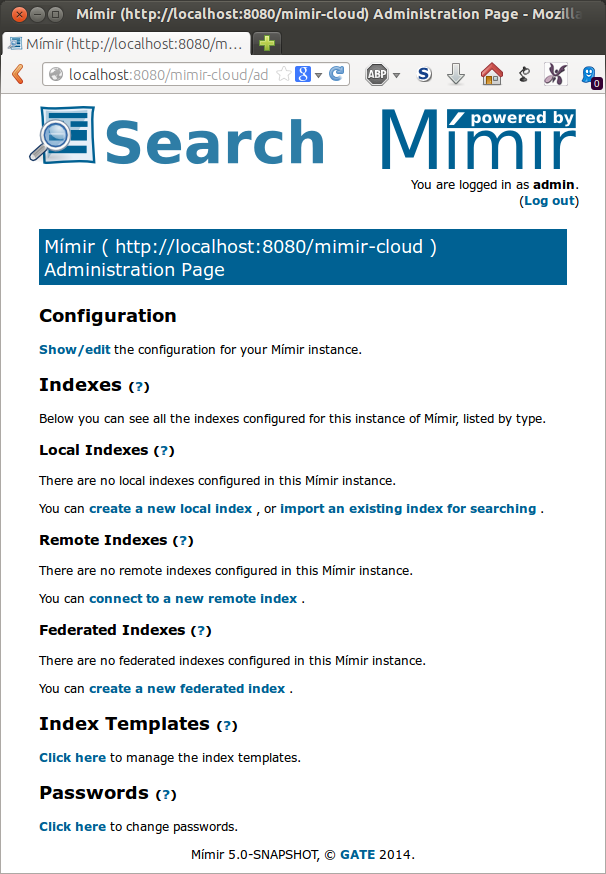
\includegraphics[scale=0.5]{img/default-front-page}
\end{center}
\caption{The default front page of a new \Mimir}
\label{fig:front-page}
\end{figure}
%
The {\em index templates} mentioned at the bottom, are used to define the
properties of new indexes, and are described in more detail in
Chapter~\ref{sec:indexing}.  The \Mimir\ Grails plugin provides a single
example template based on ANNIE annotation types.

To create an empty local index ready to receive documents for indexing, select
the {\em create a new local index} link.  This will present a form
(Figure~\ref{fig:new-local-index}) asking for the name of the new index and the
template from which it should be created.  The ``Document URIs are external
links'' option affects the way documents are presented in the search interface.
Every document in \Mimir\ is identified by a URI, and if you intend to use
document URIs that are actually resolvable URLs (for example if your documents
came from a web crawl) then you should select this option to add a link to the
original document to the search results.  If the document URIs will not be
resolvable URLs then leave the option un-selected.
%
\begin{figure}[htb!]
\begin{center}
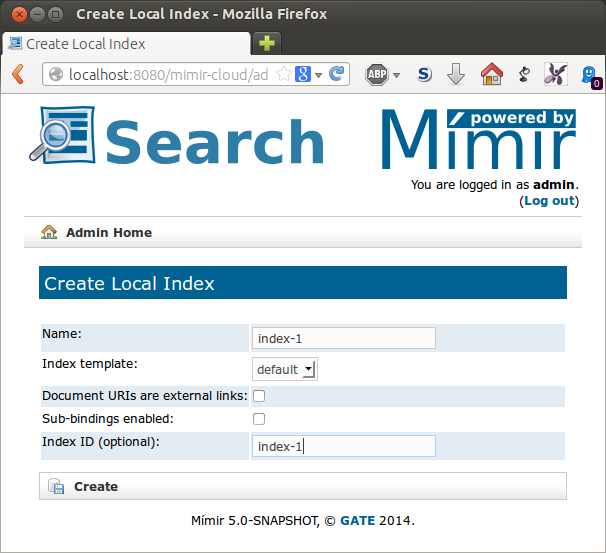
\includegraphics[scale=0.5]{img/new-local-index}
\end{center}
\caption{Creating a new local index}
\label{fig:new-local-index}
\end{figure}
%
The index will be assigned a unique identifier and a new directory will be
created under the \verb|indexBaseDirectory| you configured earlier to
hold the index data.  The newly-created index will start in the {\em ready}
state (see Figure~\ref{fig:local-index-created}), ready to receive documents
for indexing.  For details of how to submit documents to the index, see
Chapter~\ref{sec:indexing}.
%
\begin{figure}[htb!]
\begin{center}
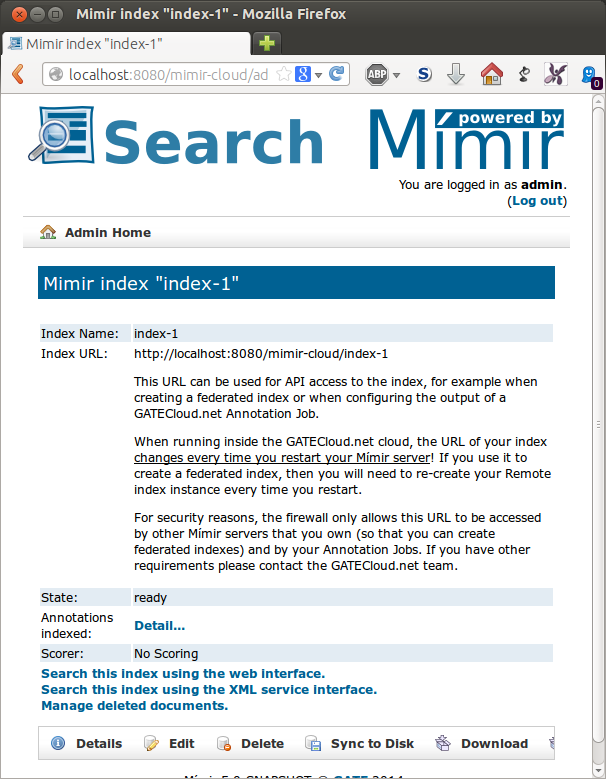
\includegraphics[scale=0.5]{img/local-index-created}
\end{center}
\caption{Results of creating a new local index}
\label{fig:local-index-created}
\end{figure}
%

This {\em index information} page can be accessed at any time by clicking the
link for the relevant index name from the \Mimir\ front page
(Figure~\ref{fig:local-index-list}).
%
\begin{figure}[htb!]
\begin{center}
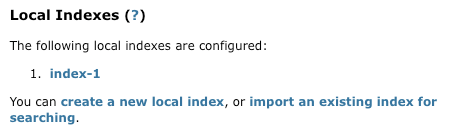
\includegraphics[scale=0.5]{img/local-index-list}
\end{center}
\caption{List of local indexes on the \Mimir\ front page}
\label{fig:local-index-list}
\end{figure}
%
At any time, the index can then be searched using the tools described in
Chapter~\ref{sec:searching}. Recently added documents only become avaialble for
searching after a {\em sync-to-disk} has taken place. Sync operations happen
automtaically at regular intervals, or can be triggered by the user by pressing
the {\em Sync to Disk} button seen at the bottom of the index information page.

\subsection{Working with Remote and Federated Indexes}

The architecture of \Mimir\ is designed to make working with remote and
federated indexes as transparent as possible.  The setup process will obviously
vary for the different index types, but once created the process of submitting
documents for indexing or of performing queries is exactly the same for all
indexes.

\subsubsection{Remote indexes}\label{sec:admin:remote-index}
A {\em remote} index is a mechanism whereby one \Mimir\ instance can
transparently index documents in, or send queries to, an index that is located
in a different \Mimir\ instance, typically running on separate hardware.  To
connect one {\em master} \Mimir\ instance to an index running in another {\em
slave} instance, first visit the index information page for the relevant
index on the slave and make a note of its {\em remote URL} (typically a URL of
the form \verb|http://server:port/mimir/remote/{UUID}|).  Now on the front page
of the master instance, select the {\em connect to a new remote index} link.
This will present a form (Figure~\ref{fig:connect-remote-index}) asking for a
name for the remote index (which need not be the same as the name of the index
on the slave), and a {\em remote URL} which is the one you made a note of from
the slave above. You should never create a remote index pointing to another
index in the same \Mimir\ instance. Such a configuration is not supported and
will lead to errors!
\begin{figure}[htb!]
\begin{center}
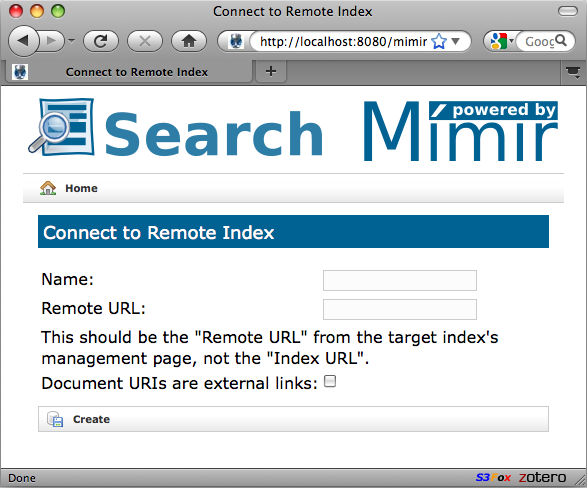
\includegraphics[scale=0.5]{img/connect-remote-index}
\end{center}
\caption{Connecting to a remote index}
\label{fig:connect-remote-index}
\end{figure}
%

The remote index defined on the master server will synchronise its state with
that of the underlying index on the slave, and once created will be usable
exactly like a local index.  However remote indexes are rarely used directly,
as in most cases it is more efficient to operate on the slave instance
itself.  The main benefit of remote indexes comes when they are used as part
of a {\em federated index}.

\subsubsection{Federated indexes}

A {\em federated index} is a device to bundle several indexes (which can
themselves be local, remote or federated) together so they can be used as a
single index.  Documents for indexing are shared out between the component
{\em sub-indexes}, and searches are performed by all sub-indexes in parallel.
Thus a federation of five indexes each containing 200,000 documents will
typically run queries faster than a single index containing 1 million
documents.  To create a federated index, go to the \Mimir\ front page and
select the {\em create a new federated index} link.  This will present a form
(Figure~\ref{fig:new-federated-index}) asking for a name for the federated
index.  The form also includes a multiple-selection list to specify the
sub-indexes to be included in the federated index.  Select the appropriate
entries from this list using the usual multiple list selection mechanism
(ctrl-click on Windows or Linux, cmd-click on Mac OS X) and press the
{\em Create} button to create the index.
%
\begin{figure}[htb!]
\begin{center}
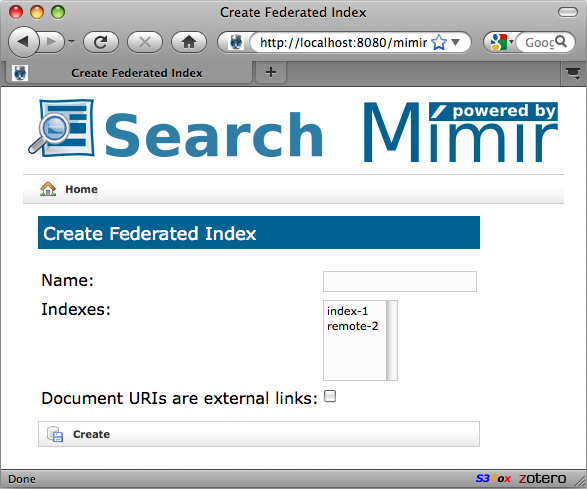
\includegraphics[scale=0.5]{img/new-federated-index}
\end{center}
\caption{Creating a new federated index}
\label{fig:new-federated-index}
\end{figure}
%
Once created the federated index will be usable exactly like a local or remote
index.

\subsection{Deleting Indexes}

If an index registered with Mimir is no longer required it can be deleted by
selecting the {\em Delete} button from the index information page (accessible by
clicking on the name of the relevant index on the \Mimir\ front page).  For
remote and federated indexes this simply deletes the ``registration'' of the
index with \Mimir, which can be easily re-created as above.  For local indexes
it also offers the option to delete the underlying index files from disk.  If a
local index is deleted without deleting the disk files then the index can be
re-created later using the {\em import an existing index for searching} option
from the \Mimir\ front page.

\Mimir\ will not allow the deletion of an index which is currently part of a
federated index in the same \Mimir\ instance.  To delete such an index, it must
first be removed from the federated index.  This guarantee only applies to
indexes within a {\em single} \Mimir\ instance --- \Mimir\ does not prevent the
deletion of an index on a slave instance which is being used as a remote index
by a master instance (it prevents the deletion of the remote index definition
in the master but not the slave index it points to).  However to do so would
put the remote index on the master (and hence any federated index that it is
part of) into the {\em failed} state, preventing further use until the problem
is resolved.

\section{``Deleting'' Documents from a \Mimir\ Index}\label{sec:admin:takedown}

While \Mimir\ indexes are not directly modifiable once they have been created,
there are situations in which it is necessary to remove documents that should
not have been indexed in the first place, or documents that may be considered
libellous, etc.  To support this, \Mimir\ provides a mechanism to mark
individual documents in the index as ``deleted'', and any documents so marked
will be excluded from future queries.  It is not possible to completely delete
the data from the index files on disk, short of completely re-building the
index from scratch, but documents marked as deleted are not accessible through
any of the public \Mimir\ APIs or user interfaces.

To mark a document as deleted (or to remove an existing deletion marker, making
the document available for queries again), use the ``Manage deleted documents''
link from the index's administration page.  This will present the screen shown
in figure~\ref{fig:deleted-documents}, with a text box into which you can type
one or more (space-separated) document IDs, and choose whether to mark them as
deleted or as ``not deleted'' (i.e. to remove any existing deletion markers for
those document IDs).
%
\begin{figure}[htb!]
\begin{center}
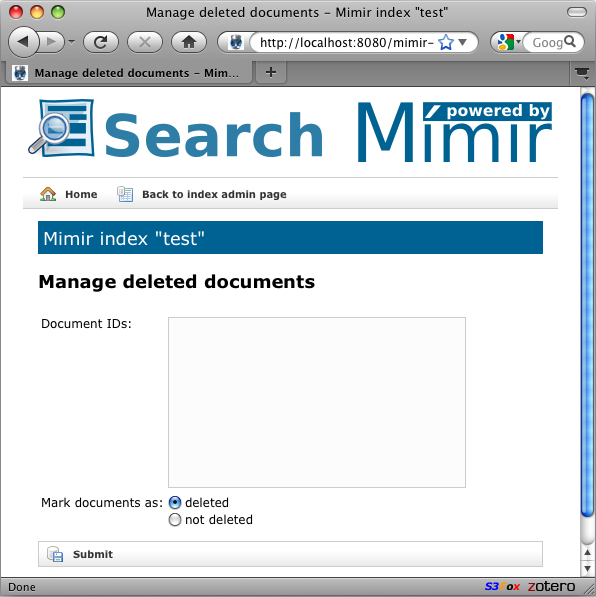
\includegraphics[scale=0.5]{img/deleted-documents}
\end{center}
\caption{Managing deleted documents}
\label{fig:deleted-documents}
\end{figure}

Note that the IDs required here are not the URIs that were provided with the
documents when they were indexed, but the internal \Mimir\ document IDs which
are numbers starting from 0, as returned in the hit lists and ``getDocumentId''
by the \Mimir\ query APIs (see section~\ref{sec:search:service}).

\chapter{Indexing Documents with \Mimir}\label{sec:indexing}
\Mimir\ is designed to index semantically annotated documents. It accepts as
input GATE documents\footnote{\url{http://gate.ac.uk/userguide/chap:corpora}}
and produces a set of indexes as a result. The way the text and annotations of
the input documents are converted into indexes is controlled through
configuration options.

\section{Configuring the indexer}

In the \Mimir\ web interface, the configuration of a new index is represented
by an {\em index template}.  This specifies:
\begin{itemize}
\item which annotation types and features to index
\item which annotation sets contain these annotations
\item how to handle the document format and metadata
\end{itemize}

Index templates can be managed using the ``Click here to manage the index
templates'' link at the bottom of the \Mimir\ front page.  An index template is
specified in a structured ``domain specific language'' using Groovy ---
Listing~\ref{lst:default-index-template} shows an example of the default
template provided by the \Mimir\ Grails plugin.
%
% Define a new command for the default index template so we can slice it up
% lower down
%
\newcommand{\defaultIndexTemplate}[1][]{{%
  \lstset{morecomment=[is]{/@}{@/}}%
  \lstinputlisting[breaklines, breakindent=150pt, #1]{default-index-config.txt}%
}}%
%
\defaultIndexTemplate[float=htb,%
    caption={The default index template provided with \Mimir},%
    label=lst:default-index-template,%
]

{\newpage}
The various sections of the template are as follows:

\subsection*{Imports}
\defaultIndexTemplate[linerange=1-3,firstnumber=1]

The template can optionally start with import statements to import any Java
classes that are used further on in the template.

\subsection*{Token definitions}\label{sec:indexing:tokens}
\defaultIndexTemplate[linerange=5-11,firstnumber=5]

The next section of the template deals with the {\em tokens} that \Mimir\ will
base its index on.  \Mimir\ sees every document as a stream of tokens rather
than a stream of characters, and all the annotations indexed by \Mimir\ are
stored in terms of their starting and ending {\em tokens}, not character
offsets.  Thus for \Mimir\ to work correctly it needs to know how to split up
the document into tokens and what information to store about each token.  For
this purpose it uses GATE annotations, and indexes the values of features on
the annotations.

The following options can be configured:
\begin{description}
\item[tokenASName] The name of the annotation set in which the token
  annotations can be found.  This may be left unspecified (or explicitly set to
  \lstinline!null!, without quotes) to use the default annotation set, which
  has no name.
\item[tokenAnnotationType] The annotation type that should be used as tokens.
  This entry is required, and can generally be simply set to the default
  \lstinline!ANNIEConstants.TOKEN_ANNOTATION_TYPE! (with a suitable
  \lstinline!import! at the top of the template).
\item[tokenFeatures] A block of code giving the features from each token
  annotation that should be indexed.
\end{description}

The {\em tokenFeatures} block should list the features to be indexed as shown
in the example, each feature name followed by parentheses.  For advanced users
an MG4J \lstinline!TermProcessor! instance may be provided inside these
parentheses.  By default, if no term processors are specified, the {\em first}
feature is converted to lowercase and the subsequent features are not modified.
Since terms in a query are processed using the same processor as those in the
index, this has the effect of making searches on the first feature
case-insensitive, and searches on the other features case-sensitive. To stop
any processing being done, you should supply a
\lstinline!it.unimi.dsi.mg4j.index.NullTermProcessor! value, by specifying e.g.
\lstinline!string(NullTermProcessor.getInstance())!, after including the
relevant \lstinline!import! statement at the top.

\subsection*{Semantic annotations}\label{sec:indexing:helpers}
\defaultIndexTemplate[linerange={13-17},firstnumber=13]

The next section defines the {\em semantic annotations} that \Mimir\ will
include in the index.  Each \lstinline!index! block defines a set of semantic
annotation types that will be indexed and stored together in one index.  The
choice of how to group annotation types together into indexes can affect the
indexing speed, as the annotations within one index are processed sequentially
by a single thread, whereas types in separate indexes can be indexed in
parallel.

Each annotation type to be indexed is introduced by ``{\tt annotation}''.  This
is a method call in the Groovy DSL which takes the following named arguments:
\bde
\item[helper] The {\em semantic annotation helper} Java object that should be
  used to index this annotation type.
\item[type] The annotation type that is to be indexed.  When using the default
  semantic annotation helper types this can be omitted.\footnote{In particular,
  if the specified helper has a method ``{\tt getAnnotationType()}'' then this
  will be called and the returned value used as the annotation type.  All the
  standard helpers provided with \Mimir\ extend
  {\tt AbstractSemanticAnnotationHelper} which implements this method.}
\ede

\subsubsection{Semantic Annotation Helpers}

Semantic annotations are stored in special indexes that associate URIs with
document positions. During indexing, the role of the helper implementations is 
to store the necessary information about each annotation to be indexed in a
persistent form and return one or more URIs that identify it.

One could make a distinction between {\em generic} semantic annotation helper
types, which can be configured to handle any annotation type and features, and
{\em special-purpose} helpers that are designed to handle specific annotation
types.  \Mimir\ supplies two generic helper implementations in the {\tt db-h2}
and {\tt sesame} plugins\footnote{A third implementation in the {\tt ordi}
plugin is now deprecated.  This stores the data in the same underlying OWLIM
semantic repository format but accesses it through a different API
abstraction.} that store annotation information in a relational database and a
knowledge base respectively.  For the most standard cases, one or other of
these default helper implementations should be sufficient.  One sample
special-purpose helper for {\tt Measurement} annotations (as generated by the
GATE {\tt Tagger\_Measurements} plugin) is also provided, in the
{\tt measurements} plugin.  This is intended both to be useful in its own right
and to serve as a template for how to implement your own helpers for other
complex annotation types.  The {\tt sparql} plugin provides a helper that can
wrap any other helper and add the ability to query for URI-valued features by
making a query to a SPARQL endpoint.  These plugins are discussed in detail in
chapter~\ref{sec:plugins}.

{\bf Note for users upgrading from \Mimir\ 3.2.0 and earlier:} the previous
index template DSL style using the annotation type as the method name and the
nominalFeatures etc. as parameters is still supported but should be considered
deprecated.  You should consider porting your index templates to the new style,
as support for the old style may be removed in a future release.

\subsection*{Document rendering and metadata}
\defaultIndexTemplate[linerange={25-26},firstnumber=25]

The final part of the template concerns how document-level metadata is indexed,
and how this can be combined with the document text to render the document
content at search time, with matches of the query highlighted.  These tasks are
performed by objects that implement the interfaces
\lstinline!DocumentMetadataHelper! and \lstinline!DocumentRenderer!
respectively (both in the \lstinline!gate.mimir! package). \Mimir\ provides a
single class \lstinline!gate.mimir.index.OriginalMarkupMetadataHelper!
which implements both interfaces, so in most cases the same object can be used
for both jobs.

An index template must define one \lstinline!documentRenderer! and may define
any number of \lstinline!documentMetadataHelpers! (in a square-bracketed list).
If the renderer is an \lstinline!OriginalMarkupMetadataHelper! (or a subclass)
then the renderer object must be included in the list of metadata helpers in
order to function correctly.  Other metadata helpers may be added to the list
if required.

\section{Adding Documents to an Index}\label{sec:indexing:add-docs}

Once an index has been created in {\em indexing} mode, the next stage is to add
documents to the index.  \Mimir\ provides an HTTP API for this which accepts
documents for indexing via HTTP POST requests that include the document in Java
serialised format.  The easiest way to make use of this API is via GCP (the
GATE Cloud Paralleliser batch processing tool) using a
\lstinline!MimirOutputHandler!.  This GCP output handler makes use of the
\lstinline!gate.mimir.index.MimirConnector! (in the {\tt mimir-client} module)
to actually make the remote call, and you can use the same API in your own
code.  To add a GATE document to an open index simply call:
\begin{lstlisting}[breaklines]
MimirConnector.defaultConnector().sendToMimir(document, uri, indexUrl);
\end{lstlisting}
%
\ldots{}with the following parameters:
\bde
\item[document] a \lstinline!gate.Document! for indexing.
\item[uri] the URI that should be used to identify the document in the \Mimir\
  index.  May be \lstinline!null!, in which case \Mimir\ will generate a URI,
  but in most cases there will be a more meaningful identifier that could be
  used.
\item[indexUrl] a \lstinline!java.net.URL! pointing to the location of the
  \Mimir\ index.  This is the ``Index URL'' given on the index information page.
\ede

The document to be indexed must, of course, contain the token and semantic
annotations that the index expects.

It is possible to create your own private instance of
\lstinline!MimirConnector! rather than simply using the default one, but this
is not necessary in normal use.

\section{The default representation scheme}\label{sec:indexing:dsah-detail}

\begin{figure}[htb]
\begin{center}
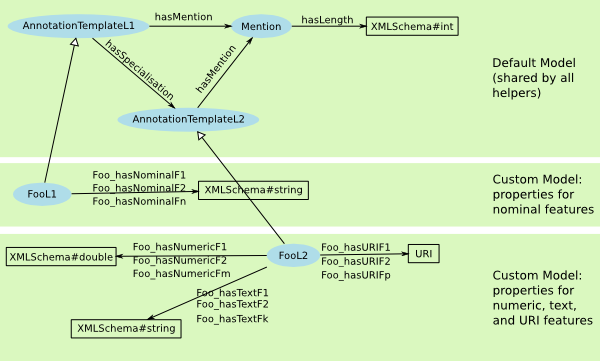
\includegraphics[scale=0.66]{img/dsah-model}
\caption{Default semantic annotation helper representation schema.}
\label{fig:dsah-model}
\end{center}
\end{figure}

The default generic SAH implementations try to minimise the amount of data stored in their underlying database or semantic repository
by creating representation templates that are shared
between all occurrences of annotations with the same values for the features.
There are two levels of templates, the first defined by the values of nominal
features, and the second that uses the values of all the other features. This
is intended to reflect the typical scenario where most annotations are defined
by a small set of nominal features, with a few of them having features with
arbitrary values. Most annotation types would then only make use of level-1
templates, with a few of them employing both level-1, and level-2 templates.

\begin{figure}[htb]
\begin{center}
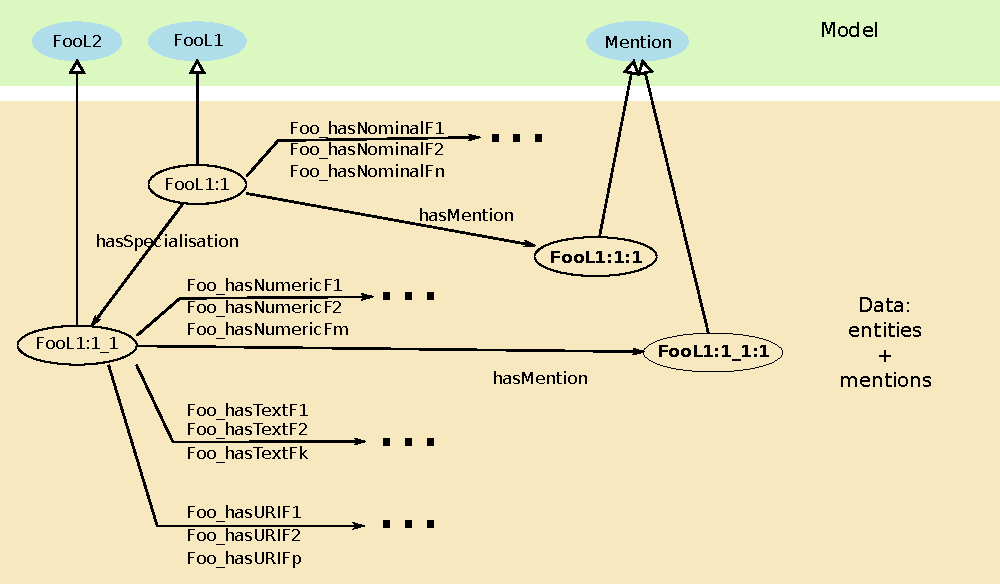
\includegraphics[scale=0.66]{img/dsah-data}
\caption{Default semantic annotation helper data example.}
\label{fig:dsah-data}
\end{center}
\end{figure}

The representation schema used by the Sesame helper is illustrated in
Figure~\ref{fig:dsah-model}.  Figure~\ref{fig:dsah-data} shows the data created
for an example annotation, with the two mention URIs displayed in bold. These
URIs will be stored in the mentions index.  The DB helper uses a similar
strategy, with separate level 1 (nominal) and level 2 (everything else)
database tables for each annotation type.  Annotation types that only have
nominal features need just a level 1 table.

The execution flow for each annotation includes the following main steps:
\bit
  \item Given the annotation's nominal features, find an appropriate level-1
  (L1) template. If none is found, create one.
  \item For the L1 template, find a mention of appropriate length (the number
  of tokens covered by the annotation). If none is found, create one. Add the
  mention URI to the mentions index.
  \item If the annotation has non-nominal features:
  \begin{itemize}
    \item Find an appropriate level-2 (L2) template, based on the feature
    values. If none is found, create one.
    \item For the L2 template, find (or create) a mention of appropriate length;
    add the mention URI to the index.
  \end{itemize}  
\eit

All annotations sharing the same feature values will share the same database
entries or knowledge base entities (the resources with URIs `\verb!FooL1:1!'
and `\verb!FooL1:1_1!'), and the same mention objects. This has the
advantage of reducing the size of the database, which allows more
documents to be indexed, and helps achieve better execution speeds during
search. The downside of this is that the indexing process is somewhat slowed
down, as pre-existing entities need to be retrieved at every step.

\chapter{Searching \Mimir\ Indexes}\label{sec:searching}
From a user's point of view, \Mimir\ is a tool for searching a collection of
semantically annotated documents.  It provides facilities for searching over
different views of the document text, for example one can search the document
words, the part-of-speech of those words, or their morphological roots. Beside
searching the document text, \Mimir\ also supports searches over the documents'
semantic annotations, where queries are based on annotation types and
restrictions over the values of annotation features. These different search
paradigms can be combined freely into complex queries, with support for
sequences, repetitions, and Boolean operators.

A search session entails the formulation of a query, running the query with the
\Mimir\ query engine, and consuming the query results.  \Mimir\ queries are
expressed in a text-based query language which is described in
section~\ref{sec:search:ql}.  The way these queries are submitted to \Mimir\
depends on how it is deployed, the various interfaces are discussed in
section~\ref{sec:search:interfaces}.


\section{The \Mimir\ query language}\label{sec:search:ql}

A \Mimir\ query is either a simple query (i.e. a {\tt String} query,
section~\ref{sec:string-query}, or an {\tt Annotation} query,
section~\ref{sec:annotation-query}), or a compound one, which comprises a set of
sub-queries linked by operators. If no operator is placed between any two
sub-queries, then the {\tt Sequence} operator (see
section~\ref{sec:sequence-query}) is implied. This means that several queries
written one after another are interpreted as one sequence query. For example, a
query like `{\it the brown dog}' is interpreted as a sequence query, having
three sub-queries, each of them being a String query. This would match
occurrences of the exact phrase `{\it the brown dog}' in the indexed documents.
Note that this is different from the standard behaviour of search engines,
which would simply match documents in which all three query terms occur, in
whichever order. That type of search is also supported in \Mimir, through the
{\tt AND} operator (see section~\ref{sec:and-query}).  Parentheses can be used
for grouping where the syntax would otherwise be ambiguous.

\subsection{String Queries}\label{sec:string-query}

The simplest form of query is a query term. This will match all occurrences of
the query term in the indexed documents.

If the \Mimir\ index being interrogated includes multiple token indexes, then
the particular index to be searched can be specified by prefixing the query
term with the index name and a colon, for example the query
`{\it root:be}'\footnote{This assumes that an index named {\tt root} exists,
and was used to store the morphological root of the words.} will match all
morphological forms of the verb {\it to be}. If the name of the string index is
omitted, then the first configured index is used. By convention (reflected in
the default \Mimir\ configuration) the first string index is used to store the
terms text, so the default behaviour is to search over the document text, as
expected.  Double-quoted strings are treated as plain term queries against the
first token index in a similar way.

In fact the above is a slight simplification, as bare terms (and double-quoted
strings) are actually tokenised before being searched for.  This is because
\Mimir\ views documents as streams of tokens, not characters, and the query
must match the tokenisation that was used to index the documents.  For example,
the default GATE tokeniser treats ``don't'' as two tokens, ``do'' and ``n't'',
so a query for {\em don't} as a single token would fail.  To get around this,
\Mimir\ runs a GATE application over the string of the query to generate
Token annotations, and then constructs a query for these tokens in sequence
(see section~\ref{sec:sequence-query}).  Named index queries (``root:be'') are
not tokenised, so if you want to avoid tokenising a particular query for any
reason (e.g. if you suspect there is a mis-tokenised document in your index)
you can explicitly name the appropriate index (typically ``string'', i.e.
string:don't).

\subsubsection{Annotation Queries}\label{sec:annotation-query}

If annotation indexes were used during indexing, \Mimir\ allows searching for
annotation-based patterns. An annotation is a piece of metadata
associated with a text segment, with a {\bf type} and optionally
{\bf features}.  An annotation query takes the following form: 
{\tt \{Type feature1=value1 feature2=value2 \ldots\}}.  The annotation type is
required, the feature constraints are optional.

While the example above uses equality for the feature constraints, other
operators are also available. Here is the full list:
\bde
  \item[equality:] represented by the sign $=$, matches annotations which have
  the given value for the specified feature. The equality operator is
  applicable to features of any type.
  \item[comparison operators:] represented by one of the following symbols:
  $<$, $<=$, $>$, $>=$, with the usual meaning. These operators can apply to
  features of type {\tt nominal}, {\tt numeric}, or {\tt text}.
  \item[regular expressions:] can be specified using the syntax {\tt
  REGEX(pattern, flags)}, where the {\tt pattern} represents the regular
  expression sought, and the {\tt flags} are optional, and can be used to
  change the way matching is performed. See
  \url{http://www.w3.org/TR/xpath-functions/#regex-syntax} for a full
  specification of the regular expression support. The {\tt REGEX} operator can
  only be used for {\tt nominal}, and {\tt text} features.
\ede

Examples:\\
\{Person gender $=$ female\} -- searches for annotations of type
{\tt Person}, which have a feature named {\tt gender}, with the value
{\it female}.

\{Measurement type $=$ scalar normalisedValue $>0$ normalisedValue $<10$
normalisedUnit $=$ m\} -- searches for scalar measurements, with a unit of {\it
metre}, and a normalised value between $0$ and $10$.\footnote{The extended
support for Measurement annotations is discussed further in
section~\ref{sec:extend:measurement-helper}.}

\subsection{AND Operator: ``{\tt \&}''}\label{sec:and-query}

The `{\tt AND}' (also `\&`) operator can be used to specify queries that should
match document segments that include at least one hit from each of the
sub-queries. The results returned will always be the shortest document segments
that satisfy the query.

\subsection{OR Operator: ``{\tt |}''}\label{sec:or-query}

{\tt OR} queries are used to search hits that match one of a set of alternative
query expressions. This is indicated by using the {\tt `OR'} (also`\verb!|!')
operator between the sub-queries. A query of the form {\tt Query1 | Query2} will
return hits that match either sub-query {\tt Query1} or sub-query {\tt Query2}.

\subsection{IN and OVER Operators}\label{sec:containment-query}

The operators {\tt IN} and {\tt OVER} are used to search for hits of a query
that contain, or are contained in the hits of another query. For example:
\begin{description}
\item[Query1 IN Query2] will match all the hits of {\tt Query1} that are
contained in a hit of {\tt Query2}.
\item[Query1 OVER Query2] will match all hits of {\tt Query1} that contain (are
overlapping) a hit of {\tt Query2}.
\end{description}

\subsection{Repeats Operator: ``+''}\label{sec:kleene-query}

The $+$ operator can be used to match text segments that comprise a sequence of
hits from the same sub-query. The length of the sequence is specified though a
number (representing the {\bf maximum} number of repetitions) or through two
numeric values (representing the {\bf minimum} and {\bf maximum} number of
repetitions). For example:
\bde
  \item[{\tt to+3}] will match one, two, or three repeated occurrences of the
  word {\it to}. The returned hits will be of the form ``{\it to}'', ``{\it to  
  to}'', or ``{\it to to to}'').
  \item[{\tt \{Person\}+2..5}] will match sequences of 2, 3, 4, or 5
  adjacent {\tt Person} annotations.
  \item[{\tt (\{Location locType = city\} |
  \{Location locType = country\})+3}] will match any sequence of up to
  three Location annotations where each one refers to either a city or a
  country.
\ede

Note that there is no support for a repetition count of zero (an optional
match) -- you will need to reformulate the query to cover the versions with and
without the optional match separately and combine them with an OR, for example
{\tt (term1 term2+2 term3) | (term1 term3)}.  Similarly there is no support for
unbounded wildcards ({\em n} times or more).

\subsection{Sequence Queries and Gaps}\label{sec:sequence-query}

As sequence is the default operator in \Mimir, there is no graphical sign for
it: simply writing a set of queries one after another will cause a search for
sequences of hits, one from each sub-query. For example, the query ``{\tt the
energy level}'' is actually a sequence query where the first sub-query searches
for the word ``{\it the}'', the second for ``{\it energy}'', and the last for
``{\it level}''.

It is sometimes useful to include gaps in a sequence query, that is to allow
arbitrary text fragments (of specified length) to occur in-between the hits
from some of the sub-queries. This can be done by using the gap markers ``{\tt
[n]}'', or ``{\tt [m..n]}''. These will match a sequence of length $n$, or with
a length of between $m$ and $n$ of arbitrary tokens.

For example the query ``{\tt the [2] root:time}'' will match phrases like ``{\it
the best of times}'' or ``{\it the worst of times}'', whereas the query ``{\tt
the [2..10] root:time}'' would also match ``{\it the best use of one's time}''
(where the gap consists of six tokens -- five words and an apostrophe).

\subsection{Escaping Reserved Words}

Some words are part of the query language definition so they cannot be used
directly as query terms. If that is desired, then these constructs must be
escaped as shown in the following table:
\begin{center}
\begin{tabular}{|l|l|}
\hline
{\bf Reserved input} & {\bf Escaped form}\\
\hline \hline
\{, \} &  $\backslash$\{, $\backslash$\}\\
\hline
(, )  & $\backslash$(, $\backslash$) \\
\hline
[, ] & $\backslash$[, $\backslash$]\\
\hline
: &  $\backslash$: \\
\hline
+ &  $\backslash$+ \\
\hline
{\tt |} &  $\backslash${\tt |} \\
\hline
{\tt \&} &  $\backslash${\tt \&} \\
\hline
? &  $\backslash$? \\
\hline
$\backslash$ &  $\backslash$$\backslash$ \\
\hline
. &  $\backslash$. \\
\hline
" &  $\backslash$" \\
\hline 
=  & $\backslash$= \\
\hline
IN & ``IN'' \\
\hline
OVER & ``OVER''\\ 
\hline
OR & ``OR''\\ 
\hline
AND & ``AND''\\ 
\hline
\end{tabular}\\
\vspace{1ex}
Escaping reserved constructs in the \Mimir\ query language
\end{center}

\subsection{Semantic queries with the {\tt sesame} plugin}

If you are using the {\tt sesame} semantic annotation helper plugin, and have a
URI-valued feature named ``inst'' on your annotations, then the helper provides
an additional ``synthetic'' feature named {\tt semanticConstraint} that
provides a way to query for annotations based on information in the knowledge
base.
\begin{lstlisting}[breaklines]
{Organization semanticConstraint = "?inst <http://proton.semanticweb.org/2005/04/protont#locatedIn> <http://example.com#Sheffield> ."}
\end{lstlisting}

The value of the semanticConstraint feature is a SPARQL fragment that has
access to the {\tt ?inst} variable, referring to the URI in the ``inst''
feature of the annotation.  Clearly, the semanticConstraint mechanism is not
intended for direct use by end-users, but rather for use by other tools that
build \Mimir\ queries automatically.

%%%%%%%%%%%%%%%%%%%%%%%%%%%%%%%%%%%%%%%%%%%%%%%%%%%%%%%%%%%%%%%%%%%%%%%%%%

\section{Search interfaces -- how to submit queries to \Mimir}
\label{sec:search:interfaces}

The \Mimir\ Grails plugin supplies two search interfaces by default, with the
infrastructure to implement other interfaces as required.  An XML-based service
interface allows other applications to submit queries to the indexes hosted by
a \Mimir\ web application by POSTing requests over HTTP (described in
section~\ref{sec:search:service}).  There is also an example user-facing search
interface called {\em GUS}, intended primarily for testing and demonstration
purposes (described in section~\ref{sec:search:gus}).  Both of these interfaces
interact with the underlying indexes through the {\tt SearchService} Grails
service provided by the plugin.  When embedding the \Mimir\ Grails plugin in
another Grails application this service is the primary means for application
code to interact with \Mimir, and is described in
section~\ref{sec:search:grails}.

\subsection{\Mimir\ Search Web Service}\label{sec:search:service}

The \Mimir\ web application exposes the search functionality as a web service
that can be accessed through a simple HTTP interface. All requests are performed
by calling an action with a set of parameters; the results of a call are encoded
in XML and returned as the response to the request.  All the example URLs in
this section assume the {\tt demo-web-app} application with its default URL
mappings, running on {\tt localhost} port 8080.

The \Mimir\ web service can be accessed at a URL like:\\
{\tt http://localhost:8080/mimir-demo/\{index ID\}/search/\{action\}},
where the {\tt action} value is the name of one of the supported actions,
described below. The actual URL (with the correct index ID included) can be
obtained from the {\em index information page} presented by  the \Mimir\ web
application.  Parameters may be supplied as query parameters with a {\tt GET}
request or in normal {\tt application/x-www-form-urlencoded} form in a
{\tt POST} request.  Alternatively, they may be supplied as XML (if the request
content type is {\tt text/xml} or {\tt application/xml}) of the form:
\begin{verbatim}
<request xmlns="http://gate.ac.uk/ns/mimir">
  <firstParam>value</firstParam>
  <secondParam>value</secondParam>
</request>
\end{verbatim}

The first request to the service will return a session cookie, which must be
passed back with all subsequent requests.

When accessing the service URL with no value provided for {\tt action}, a help
page will be returned presenting the documentation associated with the XML web
service.

% Switch to compact listings mode
\lstcompact\

The following actions are available:\\
\begin{longtable}{|p{1.8cm}|p{10.2cm}|}
\multicolumn{2}{l}{\tt \bf help}\\
\hline
Function & Obtain service documentation.\\
\hline
Parameters & none\\
\hline
Returns & A help message describing how to use the service.\\
\hline
\end{longtable}

\begin{longtable}{|p{1.8cm}|p{10.2cm}|}
\multicolumn{2}{l}{\tt \bf postQuery} \\
\hline
Function & Starts a new query.  The query will execute asynchronously in a
background thread, and will initially run until it has found a maximum of 1
million hits or has been running for 30 seconds, whichever comes first.  If the
query runner hits one of these limits before the search is complete it can be
restarted by calling the {\tt getMoreHits} action. \\
\hline
Parameters & \begin{minipage}[t]{10.2cm}
\begin{description}
\item[queryString:]the text of the query, using the \Mimir\ query language.
\end{description}
\end{minipage}\\
\hline
Returns & \begin{minipage}[t]{10.2cm}
An XML message with the ID of the new query,
or an error message if there were any problems while parsing the query.

Example request:\\
\lstinline[language=XML]!http://localhost:8080/mimir-demo/a4300d00-2dd1-4797-8eaa-e65b0c7d879b/search/postQuery?queryString=%22the%22!

Example response:
\begin{lstlisting}[language=XML]
<?xml version="1.0"?>
<message xmlns='http://gate.ac.uk/ns/mimir'>
  <state>SUCCESS</state>
  <data>
    <queryId>a28656e2-18f4-4b58-b9d3-9a9378eb14d0</queryId>
  </data>
</message>
\end{lstlisting}
\end{minipage}\\
\hline
\end{longtable}

\begin{longtable}{|p{1.8cm}|p{10.2cm}|}
\multicolumn{2}{l}{\tt \bf hitCount} \\
\hline
Function & Obtains the number of hits collected so far. If a query is not
complete, more hits may be available at later time. If a query has stopped being
active before completing, it can be restarted by calling {\tt getMoreHits}.\\
\hline
Parameters & \begin{minipage}[t]{10.2cm}
\begin{description}
\item[queryId:]the ID for the query, as returned by the {\tt postQuery} action.
\end{description}
\end{minipage}\\
\hline
Returns & \begin{minipage}[t]{10.2cm}
An XML message encapsulating a numeric value, or an error message if there were 
any problems.

Example request:\\
\lstinline[language=XML]!http://localhost:8080/mimir-demo/a4300d00-2dd1-4797-8eaa-e65b0c7d879b/search/hitCount?queryId=a28656e2-18f4-4b58-b9d3-9a9378eb14d0!

Example response:
\begin{lstlisting}[language=XML]
<?xml version="1.0"?>
<message xmlns='http://gate.ac.uk/ns/mimir'>
  <state>SUCCESS</state>
  <data>
    <value>6257</value>
  </data>
</message>
\end{lstlisting}

Example error response:
\begin{lstlisting}[language=XML]
<?xml version="1.0"?>
<message xmlns='http://gate.ac.uk/ns/mimir'>
  <state>ERROR</state>
  <error>Query ID a28656e2-18f4-4b58-b9d3-9a9378eb14d1 not known!</error>
</message>
\end{lstlisting}
\end{minipage}\\
\hline
\end{longtable}

\begin{longtable}{|p{1.8cm}|p{10.2cm}|}
\multicolumn{2}{l}{\tt \bf docCount} \\
\hline
Function & Obtains the number distinct documents that have been found so far
to contain hits.\\
\hline
Parameters & \begin{minipage}[t]{10.2cm}
\begin{description}
\item[queryId:]the ID for the query, as returned by the {\tt postQuery} action.
\end{description}
\end{minipage}\\
\hline
Returns & \begin{minipage}[t]{10.2cm}
An XML message encapsulating a numeric value, or an error message if there were 
any problems.

Example request:\\
\lstinline[language=XML]!http://localhost:8080/mimir-demo/a4300d00-2dd1-4797-8eaa-e65b0c7d879b/search/docCount?queryId=a28656e2-18f4-4b58-b9d3-9a9378eb14d0!

Example response:
\begin{lstlisting}[language=XML]
<?xml version="1.0"?>
<message xmlns='http://gate.ac.uk/ns/mimir'>
  <state>SUCCESS</state>
  <data>
    <value>11</value>
  </data>
</message>
\end{lstlisting}
\end{minipage}\\
\hline
\end{longtable}

\begin{longtable}{|p{1.8cm}|p{10.2cm}|}
\multicolumn{2}{l}{\tt \bf docStats} \\
\hline
Function & Obtains the statistics for the documents that have been found so far
to contain hits. These include the document IDs and the number of hits for
each individual document.\\
\hline
Parameters & \begin{minipage}[t]{10.2cm}
\begin{description}
\item[queryId:]the ID for the query, as returned by the {\tt postQuery} action.
\item[startIndex]the first requested document. A value of $0$ requests the
details for the first document found to contain hits.
\item[count]the number of documents for which the details are requested.  
\end{description}
\end{minipage}\\
\hline
Returns & \begin{minipage}[t]{10.2cm}
An XML message encapsulating a set of {\tt <document>} elements, one for
each individual document.

Example request:\\
\lstinline[language=XML]!http://localhost:8080/mimir-demo/a4300d00-2dd1-4797-8eaa-e65b0c7d879b/search/docStats?queryId=a28656e2-18f4-4b58-b9d3-9a9378eb14d0&startIndex=0&count=11!

Example response:
\begin{lstlisting}[language=XML]
<?xml version="1.0"?>
<message xmlns='http://gate.ac.uk/ns/mimir'>
  <state>SUCCESS</state>
  <data>
    <document id='0' hitCount='622'/>
    <document id='1' hitCount='300'/>
    <document id='2' hitCount='448'/>
    <document id='3' hitCount='273'/>
    <document id='4' hitCount='1053'/>
    <document id='5' hitCount='677'/>
    <document id='6' hitCount='86'/>
    <document id='7' hitCount='1399'/>
    <document id='8' hitCount='356'/>
    <document id='9' hitCount='841'/>
    <document id='10' hitCount='202'/>
  </data>
</message>
\end{lstlisting}
Note that as our query was simply {\it ``the''}, we have found hits on every
document. In a more typical case, not all document IDs will be represented in
the results.
\end{minipage}\\
\hline
\end{longtable}

\begin{longtable}{|p{1.8cm}|p{10.2cm}|}
\newpage\multicolumn{2}{l}{\tt \bf hits} \\
\hline 
Function & Obtains a set of hits. Each hit is defined by a document
ID, a position and a length, both of which are defined in terms of tokens, not
characters (see Section~\ref{sec:indexing:tokens} for details).\\
\hline
Parameters & \begin{minipage}[t]{10.2cm}
\begin{description}
\item[queryId:]the ID for the query, as returned by the {\tt postQuery} action.
\item[startIndex]the first requested hit. A value of $0$ requests the
details for the first hit found.
\item[count]the number of hits for which the details are requested.  
\end{description}
\end{minipage}\\
\hline
Returns & \begin{minipage}[t]{10.2cm}
An XML message encapsulating a set of {\tt <hit>} elements, one for
each individual hit.

Example request:\\
\lstinline[language=XML]!http://localhost:8080/mimir-demo/a4300d00-2dd1-4797-8eaa-e65b0c7d879b/search/hits?queryId=a28656e2-18f4-4b58-b9d3-9a9378eb14d0&startIndex=0&count=11!

Example response:
\begin{lstlisting}[language=XML]
<?xml version="1.0"?>
<message xmlns='http://gate.ac.uk/ns/mimir'>
  <state>SUCCESS</state>
  <data>
    <hits>
      <hit documentId='0' position='257' length='1'/>
      <hit documentId='0' position='266' length='1'/>
      <hit documentId='0' position='290' length='1'/>
      <hit documentId='0' position='303' length='1'/>
      <hit documentId='0' position='309' length='1'/>
      <hit documentId='0' position='316' length='1'/>
      <hit documentId='0' position='320' length='1'/>
      <hit documentId='0' position='332' length='1'/>
      <hit documentId='0' position='335' length='1'/>
      <hit documentId='0' position='342' length='1'/>
      <hit documentId='0' position='348' length='1'/>
    </hits>
  </data>
</message>
\end{lstlisting}
\end{minipage}\\
\hline
\end{longtable}

\begin{longtable}{|p{1.8cm}|p{10.2cm}|}
\multicolumn{2}{l}{\tt \bf getMoreHits} \\
\hline
Function & Requests a query that has stopped collecting hits before
completing to restart collecting hits. If the query has already completed, or
is already active, this call will simply be ignored (it will not cause an
error).\\
\hline
Parameters & \begin{minipage}[t]{10.2cm}
\begin{description}
\item[queryId:]the ID for the query, as returned by the {\tt postQuery} action.
\end{description}
\end{minipage}\\
\hline
Returns & \begin{minipage}[t]{10.2cm}
An XML message reporting success or failure.

Example request:\\
\lstinline[language=XML]!http://localhost:8080/mimir-demo/a4300d00-2dd1-4797-8eaa-e65b0c7d879b/search/getMoreHits?queryId=a28656e2-18f4-4b58-b9d3-9a9378eb14d0!

Example response:
\begin{lstlisting}[language=XML]
<?xml version="1.0"?>
<message xmlns='http://gate.ac.uk/ns/mimir'>
  <state>SUCCESS</state>
</message>
\end{lstlisting}
\end{minipage}\\
\hline
\end{longtable}

\begin{longtable}{|p{1.8cm}|p{10.2cm}|}
\multicolumn{2}{l}{\tt \bf isActive} \\
\hline
Function & Checks if a query is still working on collecting hits.\\
\hline
Parameters & \begin{minipage}[t]{10.2cm}
\begin{description}
\item[queryId:]the ID for the query, as returned by the {\tt postQuery} action.
\end{description}
\end{minipage}\\
\hline
Returns & \begin{minipage}[t]{10.2cm}
An XML message encapsulating a Boolean value, or an error message if there were 
any problems.

Example request:\\
\lstinline[language=XML]!http://localhost:8080/mimir-demo/a4300d00-2dd1-4797-8eaa-e65b0c7d879b/search/isActive?queryId=a28656e2-18f4-4b58-b9d3-9a9378eb14d0!

Example response:
\begin{lstlisting}[language=XML]
<?xml version="1.0"?>
<message xmlns='http://gate.ac.uk/ns/mimir'>
  <state>SUCCESS</state>
  <data>
    <value>false</value>
  </data>
</message>
\end{lstlisting}
\end{minipage}\\
\hline
\end{longtable}

\begin{longtable}{|p{1.8cm}|p{10.2cm}|}
\multicolumn{2}{l}{\tt \bf isComplete} \\
\hline
Function & Checks if a query has finished collecting all the hits. If a query
is not complete, more hits may be available at a later time. If a query has
stopped being active before completing, it can be restarted by calling {\tt
getMoreHits}.\\
\hline
Parameters & \begin{minipage}[t]{10.2cm}
\begin{description}
\item[queryId:]the ID for the query, as returned by the {\tt postQuery} action.
\end{description}
\end{minipage}\\
\hline
Returns & \begin{minipage}[t]{10.2cm}
An XML message encapsulating a Boolean value, or an error message if there were 
any problems.

Example request:\\
\lstinline[language=XML]!http://localhost:8080/mimir-demo/a4300d00-2dd1-4797-8eaa-e65b0c7d879b/search/isComplete?queryId=a28656e2-18f4-4b58-b9d3-9a9378eb14d0!

Example response:
\begin{lstlisting}[language=XML]
<?xml version="1.0"?>
<message xmlns='http://gate.ac.uk/ns/mimir'>
  <state>SUCCESS</state>
  <data>
    <value>true</value>
  </data>
</message>
\end{lstlisting}
\end{minipage}\\
\hline
\end{longtable}

\begin{longtable}{|p{1.8cm}|p{10.2cm}|}
\multicolumn{2}{l}{\tt \bf renderDocument} \\
\hline
Function & Renders the document text and hits for a given document, in the
context of a given query. The HTML of the document is rendered directly to the
response stream of the connection.\\
\hline
Parameters & \begin{minipage}[t]{10.2cm}
\begin{description}
\item[queryId:]the ID for the query, as returned by the {\tt postQuery} action.
\item[documentId]the ID for the requested document, as returned by e.g. a call
to the {\tt docStats} action.
\end{description}
\end{minipage}\\
\hline
Returns & \begin{minipage}[t]{10.2cm}
HTML content. The hits are rendered as 
\lstinline[language=HTML]!<span class="mimir-hit">...</span>!.

Example request:\\
\lstinline[language=XML]!http://localhost:8080/mimir-demo/a4300d00-2dd1-4797-8eaa-e65b0c7d879b/search/renderDocument?queryId=a28656e2-18f4-4b58-b9d3-9a9378eb14d0&documentId=1!

Example response fragment:
\begin{lstlisting}[language=HTML, breaklines]
...
<p num="p0002">Moreover, <span class="mimir-hit">the</span> present invention further relates to a method of higher purification effective in <span class="mimir-hit">the</span> higher purification of metal which reduces <span class="mimir-hit">the</span> oxygen content caused by organic matter.</p>
...
\end{lstlisting}
\end{minipage}\\
\hline
\end{longtable}

\begin{longtable}{|p{1.8cm}|p{10.2cm}|}
\multicolumn{2}{l}{\tt \bf documentMetadata} \\
\hline
Function & Returns the title and URI associated with a document. These values
were provided at indexing time.\\
\hline
Parameters & \begin{minipage}[t]{10.2cm}
\begin{description}
\item[queryId:]the ID for the query that has returned the document ID being
used, as returned by the {\tt postQuery} action.
\item[documentId]the ID for the requested document, as returned by e.g. a call
to the {\tt docStats} action.
\end{description}
\end{minipage}\\
\hline
Returns & \begin{minipage}[t]{10.2cm}
An XML message encapsulating the two string values, or an error message if there
were any problems.

Example request:\\
\lstinline[language=XML]!http://localhost:8080/mimir-demo/a4300d00-2dd1-4797-8eaa-e65b0c7d879b/search/documentMetadata?queryId=a28656e2-18f4-4b58-b9d3-9a9378eb14d0&documentId=1!

Example response:
\begin{lstlisting}[language=XML]
<?xml version="1.0"?>
<message xmlns='http://gate.ac.uk/ns/mimir'>
  <state>SUCCESS</state>
  <data>
    <documentTitle>EP-1288339-A9</documentTitle>
    <documentURI>urn:matrixware.com:alexandria:EP-1288339-A9</documentURI>
  </data>
</message>
\end{lstlisting}
\end{minipage}\\
\hline
\end{longtable}


\begin{longtable}{|p{1.8cm}|p{10.2cm}|}
\multicolumn{2}{l}{\tt \bf documentText} \\
\hline
Function & Action for obtaining (a segment of) the text of a document.\\
\hline
Parameters & \begin{minipage}[t]{10.2cm}
\begin{description}
\item[queryId:]the ID for the query that has returned the document ID being
used, as returned by the {\tt postQuery} action.
\item[documentId]the ID for the requested document, as returned by e.g. a call
to the {\tt docStats} action.
\item[position]the position of the first returned token. This parameter is
optional; defaults to $0$ is not provided, which means the first token of the
document.
\item[length]the number of tokens to be returned. This parameter is optional,
if omitted, all the document tokens will be returned.
\end{description}
\end{minipage}\\
\hline
Returns & \begin{minipage}[t]{10.2cm}
An XML message containing the text of all the individual tokens and, if
available, the spaces between them.


This action could be used, for example, to obtain text snippets around a query
hit.

Example request:\\
\lstinline[language=XML]!http://localhost:8080/mimir-demo/a4300d00-2dd1-4797-8eaa-e65b0c7d879b/search/documentText?queryId=a28656e2-18f4-4b58-b9d3-9a9378eb14d0&documentId=1&position=100&length=10!

Example response:
\begin{lstlisting}[language=XML]
<?xml version="1.0"?>
<message xmlns='http://gate.ac.uk/ns/mimir'>
  <state>SUCCESS</state>
  <data>
    <text position='100'>25</text>
    <text position='101'>C</text>
    <space> </space>
    <text position='102'>1</text>
    <text position='103'>/</text>
    <text position='104'>08</text>
    <space> </space>
    <text position='105'>C</text>
    <text position='106'>25</text>
    <text position='107'>C</text>
    <space>   </space>
    <text position='108'>1</text>
    <text position='109'>/</text>
  </data>
</message>
\end{lstlisting}
\end{minipage}\\
\hline
\end{longtable}

\begin{longtable}{|p{1.8cm}|p{10.2cm}|}
\multicolumn{2}{l}{\tt \bf close} \\
\hline
Function & Closes a query, releasing all resources allocated for supporting
it. After a query is closed, no more actions can be performed for it. It is
important to close queries, as each running query uses up memory on the server.
Queries are also closed automatically after a period of inactivity (upon session
expiration, the time for which is defined in the configuration of the  web
application server -- this is why it is important to pass the session cookie
you received from {\tt postQuery} back to the server with subsequent calls).
\\
\hline
Parameters & \begin{minipage}[t]{10.2cm}
\begin{description}
\item[queryId:]the ID for the query, as returned by the {\tt postQuery} action.
\end{description}
\end{minipage}\\
\hline
Returns & \begin{minipage}[t]{10.2cm}
An XML message with a success or failure value.

Example request:\\
\lstinline[language=XML]!http://localhost:8080/mimir-demo/a4300d00-2dd1-4797-8eaa-e65b0c7d879b/search/close?queryId=a28656e2-18f4-4b58-b9d3-9a9378eb14d0!

Example response:
\begin{lstlisting}[language=XML]
<?xml version="1.0"?>
<message xmlns='http://gate.ac.uk/ns/mimir'>
  <state>SUCCESS</state>
</message>
\end{lstlisting}

Example failure (using the ID for an already closed query):
\begin{lstlisting}[language=XML]
<?xml version="1.0"?>
<message xmlns='http://gate.ac.uk/ns/mimir'>
  <state>ERROR</state>
  <error>Query ID a28656e2-18f4-4b58-b9d3-9a9378eb14d0 not known!</error>
</message>
\end{lstlisting}
\end{minipage}\\
\hline
\end{longtable}

% Restore normal listings mode
\lstnormal

%%%%%%%%%%%%%%%%%%%%%%%%%%%%%%%%%%%%%%%%%%%%%%%%%%%

\subsection{GUS example user interface}\label{sec:search:gus}

The GUS search tool is a browser-based search interface intended to serve as a
platform for experimentation with a \Mimir\ index, and as a demonstration of
the capabilities of the \Mimir\ framework and API.  It is written using the
Google Web Toolkit, and the source code is included in the \Mimir\ Grails
plugin.

In the demo web application with its default URL mappings, the GUS interface
for an index in searching mode is available at 
{\tt http://localhost:8080/mimir-demo/\{index ID\}/gus/search}.  The initial
page, shown in figure~\ref{fig:gus:front-page}, provides a text area into which
you can type queries in the \Mimir\ query language.  It provides
auto-completion for annotation types and features (by asking the index what
types it was configured with when it was created).

\begin{figure}[tbp]
\begin{center}
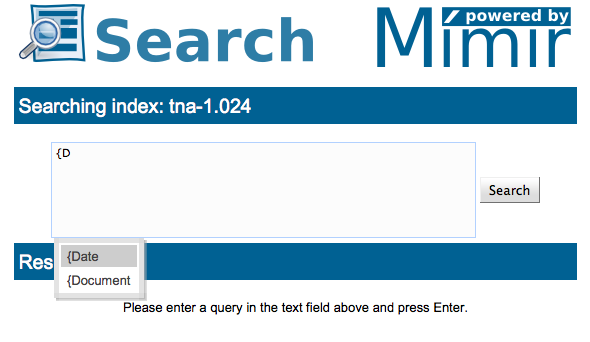
\includegraphics[scale=0.5]{img/gus-front-page}
\caption{Front page of the GUS user interface}
\label{fig:gus:front-page}
\end{center}
\end{figure}

Clicking the Search button starts a search on the server.  The query runs
asynchronously, collecting hits in the background until either 30 seconds have
passed or 1 million hits have been collected, at which point it stops.  To
restart the search, click the ``$>>$ keep searching'' link.

Hits are shown below the search box, as shown in figure~\ref{fig:gus:results},
with the hit text highlighted in bold and with five tokens of left and right
context.  The document title is a link, in this example to the original
document as the index was created with the ``Document URIs are external links''
option.  The ``cached'' link shows \Mimir's cached copy of the document, with
all the hits from that document highlighted in red.  For indexes where the
document URIs are not external links the document title would link directly to
the cached version and there would be no separate ``cached'' link.

\begin{figure}[tbp]
\begin{center}
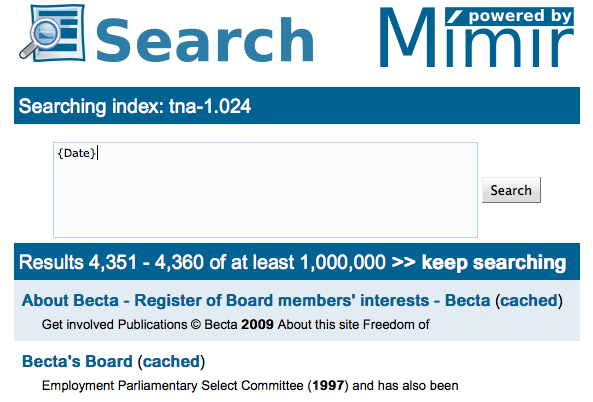
\includegraphics[scale=0.5]{img/gus-search-results}
\caption{GUS search results page}
\label{fig:gus:results}
\end{center}
\end{figure}

At the bottom of the page is a row of pagination links
(figure~\ref{fig:gus:pagination}).  Since, on a large index, there can be many
hundreds of thousands or even millions of hits to navigate, GUS provides links
where necessary to skip over large numbers of pages in one click.

\begin{figure}[tbp]
\begin{center}
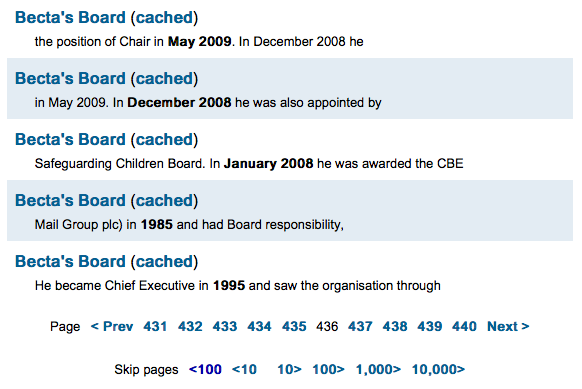
\includegraphics[scale=0.5]{img/gus-pagination-links}
\caption{GUS pagination links for a large search}
\label{fig:gus:pagination}
\end{center}
\end{figure}


%%%%%%%%%%%%%%%%%%%%%%%%%%%%%%%%%%%%%%%%%%%%%%%%%%%

\subsection{Embedding \Mimir\ in a Grails application}
\label{sec:search:grails}

Both the XML web service and the GUS interface ultimately use a Grails service
provided by the \Mimir\ plugin to search their indexes.  If you install the
\Mimir\ plugin into your own Grails application this service will be your
primary entry point to make use of \Mimir\ functionality, so this section
explains what you need to know to use it effectively.

The {\tt searchService} is a normal Grails service which can be autowired into
your own services, controllers, etc.  The service itself is very simple,
offering only the following methods:

\bde
\item[postQuery(index, queryString)] start running a query against the given
  index.  The index can be specified either as a string containing the indexId
  (the last component of the index URL, typically a UUID) or as an {\tt Index}
  domain object (the database object representing a local, remote or federated
  index).  Returns a {\em query ID} string.
\item[getQueryRunner(queryId)] retrieves the {\tt QueryRunner} for the given
  running query ID.  {\tt QueryRunner} is the interface through which you can
  interact with the running query.
\item[closeQueryRunner(queryId)] indicates that the given query runner is no
  longer required.  It is important to call this method when you have finished
  with a query runner, as each runner owns resources such as background threads
  which need to be properly cleaned up.
\ede

Once a query has been started, its {\tt QueryRunner} provides access to the
statistics, the hits themselves, and the text in the matched documents.  The
most important methods are summarised below, but for full details you should
look at the interface definition itself, in the {\tt gate.mimir.search} package
of {\tt mimir-core}.  Note that the search itself is performed in a background
thread so many of the methods of {\tt QueryRunner} will return different values
over time as the search progresses.

\bde
\item[isComplete()] Checks whether the search has completely finished and there
  are definitely no more hits to be found.
\item[isActive()] Checks whether the runner is currently actively searching.
  By default a query runner keeps searching until it has either exhausted all
  the possible hits, has found a million hits since it was last restarted, or
  has been running for 30 seconds without hitting this limit.  If isActive()
  and isComplete() both return false, it means that the search hit one of these
  limits and was suspended, it can be restarted by calling getMoreHits().
\item[getHitsCount()] Gets the number of hits obtained so far. This number may
  increase at any time if the query is currently active.
\item[getDocumentsCount()] Gets the number of distinct documents that have so
  far been found to contain hits.  This number may increase at any time if the
  query is currently active.
\item[getHits(start, max)] Gets the details of some hits found by the query.
  Conceptually, a {\tt QueryRunner} can be thought of as holding a flat list of
  hits numbered from zero upwards, containing all the hits from the first
  matched document, followed by all the hits from the second matched document,
  etc.  This method retrieves a sub-list from that list, starting at the
  (zero-based) index {\em start} and containing a maximum of {\em max} entries
  (it may contain fewer if not enough hits have yet been found).  The return
  value from this method is a list of {\tt Binding} objects, each representing
  one hit.
\item[getDocumentHitsCount(documentIndex)] Gets the number of hits in the $n$th
  document that matched this query (zero-based index).  To retrieve the hits
  for a particular document you would need to sum up all the
  getDocumentHitsCount values for the preceding documents and pass that sum as
  the {\em start} parameter to getHits.
\item[getDocumentID(documentIndex)] Gets the ID in the underlying index of the
  $n$th document that matched this query.  This ID is needed to get the
  document text and metadata.
\item[getDocumentTitle/URI(id)] Gets metadata about the document with the given
  ID.
\item[getDocumentText(id, start, length)] Gets the text of the document with
  the given ID, starting at the {\em start}th token and extending for
  {\em length} tokens.  The return value is a pair of parallel string arrays,
  one containing the text of the tokens and the other containing the text
  between each token and the following one.
\item[renderDocument(id, Appendable)] Render the document content, with hits
  highlighted, using the document renderer configured for the index.  The
  content is written to the specified Appendable (a StringBuilder, Writer,
  etc.).
\ede

The getHits method returns a list of {\tt Binding} objects, which provide
several methods, the most important ones being {\tt getDocumentId} (the
document that contains the hit), {\tt getTermPosition} (the offset of the first
token covered by the hit) and {\tt getLength} (the number of tokens it
covers).

\chapter{Standard \Mimir\ Plugins}\label{sec:plugins}
\Mimir\ uses the GATE Embedded {\em CREOLE plugin} mechanism to load semantic
annotation helper classes.  A number of plugins are supplied by default with
the \Mimir\ distribution, and those plugins are described in this chapter.
Information on how to create new plugins to provide user-defined helper classes
can be found in section~\ref{sec:extend:helpers}.

\section{The {\tt db-h2} Plugin}\label{sec:plugins:db}

The {\tt db-h2} plugin a plugin that provides a {\em generic} semantic
annotation helper implementation that can be configured for any annotation type
with any features.  The helper provided by {\tt db-h2} uses an embedded
relational database engine (\url{http://www.h2database.com/}) to store the
annotation data, and generally provides the best performance of the standard
generic helpers.

\lstinline!gate.mimir.db.DBSemanticAnnotationHelper! is the helper class
provided by the {\tt db-h2} plugin.  It has a constructor that takes a
{\tt Map} of configuration parameters, and Groovy provides special ``named
argument'' support for {\tt Map}-valued method and constructor parameters,
allowing the following idiom in the index template DSL:
\begin{lstlisting}[texcl, breaklines, breakindent=150pt]
// note the ``import X as Y'', which is another Groovy feature to create an
// alias for an imported class name
import gate.mimir.db.DBSemanticAnnotationHelper as DefaultHelper
// \ldots
semanticAnnotations = {
  index {
    annotation helper:new DefaultHelper(annType:'Person',
    nominalFeatures:["gender", "title"], stringFeatures:["name"])) }
}
\end{lstlisting}

The supported constructor arguments are:
\bde
\item[annType:] the annotation type which the helper is to process.
\item[nominalFeatures:] the names of the features to be indexed that have
  nominal values. An annotation feature is said be nominal if the range of
  possible values is clearly defined and limited in size. There is no hard rule
  regarding the size of the set of permitted values, but, for optimal results,
  this should not exceed a few tens of values.
\item[integerFeatures:] the names of the features to be indexed that have
  integer values (i.e. values that can be converted to a Java {\tt long}
  value).
\item[floatFeatures:] the names of the features to be indexed that have
  floating-point numeric values (i.e. values that can be converted to a Java
  {\tt double} value).
\item[textFeatures:] the names of the features to be indexed that have
  arbitrary text values (as opposed to the nominal case of a fixed list of
  possible values).
\item[uriFeatures:] the names of the features to be indexed that have
  URIs as values.
\ede

The DB-based helper does not distinguish between text- and URI-valued features,
indexing both types in the same way, but it accepts both kinds as arguments.

\section{The {\tt measurements} Plugin}\label{sec:plugins:measurements}

The GATE {\tt Tagger\_Measurements} plugin, introduced in GATE 6.1, is able to
recognise many different kinds of measurement expressions in text.  It
normalises the value and unit of each measurement into the SI system of
measurements and stores these values as features of the Measurement annotation.
For example, the text ``45 cm'' would be annotated with a normalised unit of
metres and a normalised value of 0.45, the text ``18 in'' would also be
normalised to metres, in this case with a normalised value of 0.4572.

The \Mimir\ {\tt measurements} plugin provides a SAH that implements the same
normalisation on queries.  It processes queries for a ``synthetic'' feature
called ``spec'' which represents a measurement specification in a controlled
language and converts constraints on this feature into the corresponding
constraints on the real normalised value and unit features that have been
indexed.  For example, a search for \{Measurement spec="1 to 3 feet"\} would be
treated as a query for measurements whose normalised unit is metres and whose
normalised value is between 0.3048 and 0.9144, which would match both the ``45
cm'' and ``18 in'' examples above.

\subsection{Configuring the Measurements SAH}

To use the measurements helper you need to first ensure that the
{\tt measurements} plugin is loaded into your \Mimir\ instance, then create an
index template that specifies an instance of the helper:
\begin{lstlisting}[texcl]
import gate.mimir.measurements.MeasurementAnnotationHelper

// \ldots
semanticAnnotations = {
  index {
    // Measurement helper with default settings
    annotation helper:new MeasurementAnnotationHelper(
          delegateHelperType:DefaultHelper)
  }
}
\end{lstlisting}

Note that the measurement helper does not need any ``annType'' or
``{\em xxx}Features'' parameters, as it is hard-coded to work only for
annotations that are produced by the measurement tagger PR.  However the
constructor does take a {\tt Map} with other named arguments:
\begin{lstlisting}[firstnumber=6,texcl]
    // Example of how to configure a custom ``units'' file
    annotation helper:new MeasurementAnnotationHelper(
          delegateHelperType:DefaultHelper,
          unitsFile:'resources/americanUnits.dat',
          locale:'en_US')
\end{lstlisting}

The following parameters are supported:
\bde
\item[delegateHelperType (required)] a {\tt Class} object representing the type
  of generic helper that the Measurements helper should delegate to.  This
  class must provide a 6-argument constructor taking the annotation type (a
  String) and five String arrays for the nominal, integer, float, text and URI
  feature names respectively.
\item[unitsFile] the location of the {\tt units.dat} file used to configure the
  measurements parser.  If not specified, a default file provided with the
  {\tt measurements} plugin is used.  This value can be an absolute URL
  (file:/path/to/units.dat) or a relative path which will be resolved against
  the {\tt measurements} plugin directory.
\item[commonWords] the location of the common words file used by the
  measurements parser.  As with the {\tt unitsFile} parameter, if omitted a
  default file bundled with the plugin is used.
\item[locale] the locale under which the measurements will be parsed.  Defaults
  to ``en\_GB'' if unspecified.
\item[encoding] the character encoding used to read the configuration files.
  Defaults to ``UTF-8'' if unspecified.
\item[annType] the annotation type, if something other than the default of
  ``Measurement''
\ede

The measurements SAH is pre-configured with the feature names that the
measurements tagger produces, and attempting to specify any feature name
parameters such as nominalFeatures will cause an error.

\subsubsection{Measurements helper implementation}

The {\tt MeasurementAnnotationHelper} extends the
{\tt DelegatingSemanticAnnotationHelper} base class described above.  It does
not add any behaviour at indexing time, simply passing all the annotations
through directly to its delegate.  However it overrides the {\tt getMentions}
search method to support the ``spec'' feature.

When a query including a spec feature constraint is received, the helper parses
this spec using the measurements parser to obtain a normalised unit and value
or values for the measurement sought.  It then constructs a number of new
constraint sets that match annotations compatible with the spec and then for
each of these alternatives, runs these constraints in combination with the
other non-spec constraints of the original query against the delegate helper.
The final set of URIs returned is the union of the results obtained from the
delegate for all the alternative reformulations of the spec constraint.

As well as being useful in its own right for Measurement annotations, the
measurements helper serves as an example of how to implement your own
special-purpose helper based on the delegating base class.  Feel free to use it
as a template for your own helper implementations.

\section{The {\tt sparql} Plugin}\label{sec:plugins:sparql}

The {\tt sparql} plugin provides a semantic annotation helper that wraps
another helper, adding flexible {\em semantic query} support.  It is intended
to be used with annotations that have one or more URI-valued features whose
values refer to entities in an external knowledge base (accessible at a
standard {\em SPARQL endpoint}).  The SPARQL helper has no effect at indexing
time, simply delegating all calls through to the underlying helper, but at
search time it allows queries for the synthetic feature ``sparql''.  This
feature value is taken to be a SPARQL ``SELECT'' query, which is posted
to the configured SPARQL endpoint.  The variables in the SELECT query must
correspond to the names of features that have been indexed by the underlying
helper, and each row in the result set becomes a standard \Mimir\ query to the
underlying helper.  Any annotations that match any of these new queries will be
treated as a match for the {\tt sparql} constraint.  This process is described
in detail below.

For example, given a helper configured for the public DBPedia endpoint
{\tt http://dbpedia.org/sparql}, the following \Mimir\ query:
\begin{verbatim}
{Person sparql = "SELECT DISTINCT ?inst WHERE {
  ?inst <http://dbpedia.org/ontology/birthPlace>
    <http://dbpedia.org/resource/Sheffield> }"}
\end{verbatim}
would search for all Person annotations that have an ``inst'' feature
containing the URI of an entity in DBpedia that represents a person born in
Sheffield.


\subsection{Creating a SPARQL Helper}

The SPARQL semantic annotation helper class is called
\lstinline!gate.mimir.sparql.SPARQLSemanticAnnotationHelper!.  It has a
{\tt Map} constructor taking the following parameters:

\bde
\item[delegate (required)] the underlying semantic annotation helper that this
  SPARQL helper should wrap.
\item[sparqlEndpoint (required)] the address of the SPARQL endpoint that this
  helper should use when making SPARQL queries.
\item[queryPrefix] an optional prefix that will be prepended to the string
  specified in the {\tt sparql} synthetic feature to form the actual SPARQL
  query that will be sent to the endpoint.  Typically this would be used to
  define appropriate namespace prefixes.
\item[querySuffix] an optional suffix that will be appended to the end of the
  SPARQL queries.  Thus the actual SPARQL query submitted to the endpoint is
  {\em queryPrefix} + {\tt sparql} feature + {\em querySuffix}.
\item[sparqlEndpointUser and sparqlEndpointPassword] username and password used
  to authenticate to the SPARQL endpoint (only HTTP basic authentication is
  supported).  May be omitted if your endpoint does not require authentication.
\ede

The helper also accepts the usual ``annType'' and ``{\em xxx}Features''
parameters but these are not normally required -- if the delegate helper is a
subclass of {\tt AbstractSemanticAnnotationHelper} (which is the case for all
the standard helpers) then the SPARQL helper will take its feature names from
the delegate, so the only time the features need to be specified explicitly for
the SPARQL helper is if the delegate is a custom helper type that does not
extend {\tt AbstractSemanticAnnotationHelper}.

For example, the following configuration would set up a helper for Person
annotations operating against DBpedia, to support the example query above:
\begin{lstlisting}[texcl, breaklines, breakindent=150pt]
import gate.mimir.db.DBSemanticAnnotationHelper as DBH
import gate.mimir.sparql.SPARQLSemanticAnnotationHelper as SPARQLHelper
// \ldots
semanticAnnotations = {
  index {
    annotation helper:new SPARQLHelper(
        sparqlEndpoint:'http://dbpedia.org/sparql',
        delegate:new DBH(annType:"Person", uriFeatures:['inst']))
  }
}
\end{lstlisting}

Alternatively, the helper could be configured with a queryPrefix to set up some
useful namespace prefixes:
\begin{lstlisting}[texcl, breaklines, breakindent=150pt]
semanticAnnotations = {
  index {
    annotation helper:new SPARQLHelper(
      sparqlEndpoint:'http://dbpedia.org/sparql',
      queryPrefix:
       'PREFIX rdfs:<http://www.w3.org/2000/01/rdf-schema#> \
        PREFIX xsd:<http://www.w3.org/2001/XMLSchema#> \
        PREFIX owl:<http://www.w3.org/2002/07/owl#> \
        PREFIX rdf:<http://www.w3.org/1999/02/22-rdf-syntax-ns#> \
        PREFIX dbo:<http://dbpedia.org/ontology/> \
        PREFIX dbr:<http://dbpedia.org/resource/> ',
      delegate:new DBH(annType:"Person", uriFeatures:['inst']))
  }
}
\end{lstlisting}

Note the backslashes which are a Groovy feature to permit a String literal to
be broken across several lines, and also the trailing space before the closing
quotation mark -- the helper simply concatenates the prefix, query and suffix
without any additional space, so required spaces must be part of the prefix or
suffix string itself.  This would allow the example query above to be rewritten
more succinctly as:
\begin{verbatim}
{Person sparql = "SELECT DISTINCT ?inst WHERE {
  ?inst dbo:birthPlace dbr:Sheffield }"}
\end{verbatim}

For annotation types that have only one URI-valued feature it may be desirable
to include the ``\verb!SELECT DISTINCT ?inst WHERE { !'' in the prefix and add
a suffix of ``\verb! }!'', which would reduce the query down to
\begin{verbatim}
{Person sparql = "?inst dbo:birthPlace dbr:Sheffield"}
\end{verbatim}

If your index template includes several ontology-based annotation types sharing
the same SPARQL endpoint and prefixes then listing these in full for each
annotation type will result in a large and unwieldy template.  However, since
the index template is itself a Groovy script it is possible to declare methods
to factor out the common code.  Method declarations must be placed
{\em outside} the {\tt semanticAnnotations} block:
\begin{lstlisting}[texcl, breaklines, breakindent=150pt]
import gate.mimir.db.DBSemanticAnnotationHelper as DBH
import gate.mimir.sparql.SPARQLSemanticAnnotationHelper as SPARQLHelper

def standardHelper(type) {
  return new SPARQLHelper(
      sparqlEndpoint:'http://dbpedia.org/sparql',
      queryPrefix:
       'PREFIX rdfs:<http://www.w3.org/2000/01/rdf-schema#> \
        PREFIX xsd:<http://www.w3.org/2001/XMLSchema#> \
        PREFIX owl:<http://www.w3.org/2002/07/owl#> \
        PREFIX rdf:<http://www.w3.org/1999/02/22-rdf-syntax-ns#> \
        PREFIX dbo:<http://dbpedia.org/ontology/> \
        PREFIX dbr:<http://dbpedia.org/resource/> ',
      delegate:new DBH(annType:type, uriFeatures:['inst']))
}

// \ldots
semanticAnnotations = {
  index {
    annotation helper:standardHelper('Person')
    annotation helper:standardHelper('Location')
    annotation helper:standardHelper('Organization')
  }
}
\end{lstlisting}

\subsection{Format of SPARQL Queries}

This section describes in more detail how the SPARQL queries relate to the
annotations indexed by the underlying semantic annotation helper.  As a simple
example we consider the query for people born in Sheffield:
\begin{verbatim}
{Person sparql = "SELECT DISTINCT ?inst WHERE {
  ?inst dbo:birthPlace dbr:Sheffield }"}
\end{verbatim}
%
The helper will submit the SPARQL query to its configured endpoint, and receive
a response of the form:

\begin{tabular}{|c|}
\hline
{\bf inst} \\
\hline
{\tt http://dbpedia.org/resource/Gordon\_Banks} \\
{\tt http://dbpedia.org/resource/Michael\_Palin} \\
{\tt http://dbpedia.org/resource/David\_Blunkett} \\
\ldots \\
\hline
\end{tabular}

This will then generate a series of queries to the underlying helper of the
form:
\begin{verbatim}
{Person inst = "http://dbpedia.org/resource/Gordon_Banks"}
{Person inst = "http://dbpedia.org/resource/Michael_Palin"}
...
\end{verbatim}
and any annotation that matches any of these queries will be returned as a
match for the {\tt sparql} constraint.

The SPARQL query can bind more than one variable, and the values of the
variable bindings can be RDF literals as well as URIs, they convert to queries
on the underlying helper in the same way.

\chapter{Extending and Customising \Mimir}\label{sec:extend}
The standard semantic annotation helpers provided by \Mimir\ are adequate for
many use cases, but if your application needs more functionality that they
cannot provide it is easy to add your own custom helper implementations using a
plugin mechanism.  This process is described in
section~\ref{sec:extend:helpers}.  Similarly, the basic \Mimir\ demo
application shows the simplest way to use the \Mimir\ Grails plugin, but it
provides no authentication or security, for example.  To add these kinds of
features you can install the \Mimir\ plugin into your own custom Grails
application, as described in section~\ref{sec:extend:customapp}.

\section{Creating new Semantic Annotation Helpers}\label{sec:extend:helpers}

{\em Semantic annotation helpers} (SAHs) are the mechanism that \Mimir\ uses to
store information about annotations and allow this information to be queried at
search time.  A SAH is associated with a particular annotation type in the
\Mimir\ index configuration, and performs two functions:

\bde
\item[During indexing] for each annotation of the relevant type, store
  information about that annotation in some persistent form and return to
  \Mimir\ one or more URIs that represent that annotation.  These URIs are
  included in the main MG4J index and associated with the location
  in the document where the annotation was found.
\item[During searching] given a set of feature value constraints, use the
  persistent store created during indexing to determine the URIs associated
  with annotations that satisfy the constraints.
\ede

Conceptually, SAH implementations can be divided into two types.
{\em Generic} helpers are those that can index any annotation types and
features, and {\em special-purpose} helpers are those that are designed to work
with specific types of annotation.  There are two generic SAH implementations
provided with \Mimir\ by default.  You would create a new generic SAH
implementation if you wanted to store annotation data in a different underlying
storage format.  \Mimir\ provides one example special-purpose SAH for
Measurement annotations, which can serve as a template for how to implement
your own helpers for other annotation types.

\subsection{The {\tt SemanticAnnotationHelper} interface}

The {\tt gate.mimir.SemanticAnnotationHelper} interface is the contract that
all helpers must implement.  It specifies three groups of methods that must be
implemented:

\subsubsection*{Lifecycle methods}

The interface includes two pairs of init/close lifecycle methods, one pair
taking an {\tt Indexer} parameter (used when the helper is indexing
annotations) and the other pair taking a {\tt QueryEngine} parameter (used when
the helper is searching).  Both the Indexer and QueryEngine provide access to
an {\tt IndexConfig} object which defines the configuration of the index,
including the location of the index files on disk, and provides a mutable
``context'' map that can be used to share objects among the various SAH objects
(for example the Sesame helper uses the context to share a single connection to
the semantic repository among all the helpers associated with the index).  The
appropriate {\tt init} method is called by \Mimir\ when the index is opened (in
whichever mode), before any other requests are passed to the helper, and the
corresponding {\tt close} method is called when the index is shut down.

\subsubsection*{Indexing methods}

When indexing annotations \Mimir\ calls the following methods:

\bde
\item[documentStart(document)] Called when the indexer starts processing a
  particular document to allow the helper to perform any per-document setup
  tasks.  This method is guaranteed to be called once per document, before any
  calls to getMentionUris.
\item[getMentionUris(annotation, length, indexer)] Called once for each
  semantic annotation of this helper's type in the document.  The helper is
  expected to use the annotation's length (in tokens) and feature values to
  determine the relevant URI or URIs that represent this annotation, and return
  them. 
\item[documentEnd()] Called after all the annotation for a particular document
  have been processed.
\ede

These methods are always called from a single thread, as long as the same 
helper object is not used for more than one annotation type.

Note that the annotation length passed to {\tt getMentionUris} is measured in
{\em tokens}, not characters.  Because \Mimir\ operates on streams of tokens,
semantic annotations that partially overlap a token will be considered by
\Mimir\ to cover the whole token.  I.e. given the hypothetical example:

\begin{minipage}{\textwidth}
\begin{verbatim}
... started on 10/05/1987 by John Smith ...
    ------- -- -- -- ---- -- ---- -----
\end{verbatim}
\end{minipage}

where tokens are represented by \verb|---|, an annotation that covers just the
``87'' would be indexed as if it covered the whole ``1987'' token.

\subsubsection*{Search methods}

The final method in the interface is {\tt getMentions(annotationType,
constraints, queryEngine)}.  This method is called by \Mimir\ when searching
for annotations, and the helper must use its stored data to determine all the
possible mention URIs that satisfy the provided constraints, and return them
along with their lengths (in tokens) as provided to {\tt getMentionUris} when
the annotations were indexed.

There is a second overloading of this method specified in the interface which
is a convenience for callers when all the constraints are simple feature value
equality constraints, but generally implementors of new SAH types can ignore
this as \Mimir\ provides an abstract base class that converts the Map form of
constraints into the more general List$<$Constraint$>$ form and calls the other
method.

The {\tt getMentions()} methods may be called from multiple threads at the same
time, so implementations should be thread-safe.

\subsection{Abstract base classes}

\Mimir\ provides an abstract class {\tt AbstractSemanticAnnotationHelper}
which, as described above, implements the Map version of {\tt getMentions} in
terms of the List$<$Constraint$>$ version, and also provides empty
implementations of {\tt documentStart} and {\tt documentEnd}.  As well as this,
it provides accessor methods to access the list of feature names of each of the
five types (nominal, integer, float, text and URI) that a particular helper
object supports.  {\tt AbstractSemanticAnnotationHelper} enjoys special support
in the \Mimir\ Grails plugin, allowing clients to determine what feature names
an index supports for each annotation type whose helper extends
{\tt AbstractSemanticAnnotationHelper}.  All the standard helper
implementations provided with \Mimir\ extend this base class.

Special-purpose helpers for particular annotation types typically operate by
mapping the features of their target annotations and/or the feature constraints
in a query into a different set of features or constraints which can then be
handled by a generic helper.  The Measurement helper described in
section~\ref{sec:extend:measurement-helper} operates in this way.  To support
this pattern, \Mimir\ provides an abstract
{\tt DelegatingSemanticAnnotationHelper} which implements all the SAH interface
methods to simply delegate to another helper instance.  Subclasses can then
override the methods as appropriate to map their features or constraints into
terms that the underlying helper can understand and then call the {\tt super}
method to pass these parameters on to the delegate.

{\tt DelegatingSemanticAnnotationHelper} extends
{\tt AbstractSemanticAnnotationHelper} so it advertises the features it
supports in the usual way.  However it is important to note that the various
\verb|get*FeatureNames| methods of the delegating helper do {\em not} call
their counterparts in the delegate, which allows a delegating helper to
advertise different features from those supported by its delegate.

\subsubsection{The SAH lifecycle}

Semantic annotation helper objects go through a specific lifecycle in \Mimir.
When creating a new index for indexing, the helpers defined for each semantic
annotation type are instantiated by calling their constructors
from the Groovy DSL (see the measurements example below).
Once instantiated, the {\tt init(Indexer)} methods of each helper in turn are
called (one after the other, in a single thread, so if you are sharing objects
among your helpers through the context you can be sure that you have exclusive
access to the context map during the call to your init method).

The actual indexing process takes place in several threads in a pipelined
manner.  When a document arrives for indexing it is first processed by the
token indexer (to index the token features), then the semantic indexers
specified by the {\tt index \{ \ldots\ \}} blocks in the DSL in turn.  Each
indexer operates in its own thread, with documents passing from one to the next
via queues.  So each document is only processed by one thread at a time but
under load you may have the token indexer dealing with document 3 at the same
time as semantic indexers are dealing with documents 2 and 1.

When indexing is complete the helpers' {\tt close(Indexer)} methods are called
(again, in sequence in one thread).  The index is now closed and the SAH
objects can be garbage collected.

The index configuration, including all the SAH objects, is serialized to XML
using XStream (\url{http://xstream.codehaus.org}). Therefore it is important to
mark as \lstinline!transient! any fields of your helper class that should not be
serialized (e.g. temporary in-memory caches, etc.).

When an index is opened for searching the XML configuration is deserialized to
re-create the helper objects, and their {\tt init(QueryEngine)} methods are
called.  Note that as with Java object serialization XStream does {\em not}
call object constructors when deserializing, so any initialization must happen
in the init method or in a {\tt readResolve} method, and not in the
constructor.

Annotation queries result in calls to the relevant helper's {\tt getMentions}
method, which has been discussed in detail above.

Finally, when the index is shut down the {\tt close(QueryEngine)} methods of
the helpers are called in sequence.

\subsection{An example special-purpose helper -- the {\tt measurements} plugin}
\label{sec:extend:measurement-helper}

The GATE {\tt Tagger\_Measurements} plugin, introduced in GATE 6.1, is able to
recognise many different kinds of measurement expressions in text.  It
normalizes the value and unit of each measurement into the SI system of
measurements and stores these values as features of the Measurement annotation.
For example, the text ``45 cm'' would be annotated with a normalized unit of
metres and a normalized value of 0.45, the text ``18 in'' would also be
normalized to metres, in this case with a normalized value of 0.4572.

The \Mimir\ {\tt measurements} plugin provides a SAH that implements the same
normalization on queries.  It processes queries for a ``virtual'' feature
called ``spec'' which represents a measurement specification in a controlled
language and converts constraints on this feature into the corresponding
constraints on the real normalized value and unit features that have been
indexed.  For example, a search for \{Measurement spec="1 to 3 feet"\} would be
treated as a query for measurements whose normalized unit is metres and whose
normalized value is between 0.3048 and 0.9144, which would match both the ``45
cm'' and ``18 in'' examples above.

\subsubsection{Configuring the Measurements SAH}

To use the measurements helper you need to first ensure that the
{\tt measurements} plugin is loaded into your \Mimir\ instance, then create an
index template that specifies the right helper for Measurement annotations.
\begin{lstlisting}[texcl]
import gate.mimir.measurements.MeasurementAnnotationHelper

// \ldots
semanticAnnotations = {
  index {
    // Measurement helper with default settings
    annotation helper:new MeasurementAnnotationHelper(
          delegateHelperType:DefaultHelper)
  }
}
\end{lstlisting}

The {\tt MeasurementAnnotationHelper} constructor takes a {\tt Map} of
parameters, which can be specified in Groovy as ``named arguments'':
\begin{lstlisting}[firstnumber=6,texcl]
    // Example of how to configure a custom ``units'' file
    annotation helper:new MeasurementAnnotationHelper(
          delegateHelperType:DefaultHelper,
          unitsFile:'resources/americanUnits.dat',
          locale:'en_US')
\end{lstlisting}

The following parameters are supported:
\bde
\item[delegateHelperType (required)] a {\tt Class} object representing the type
of generic helper that the Measurements helper should delegate to.
\item[unitsFile] the location of the {\tt units.dat} file used to configure the
  measurements parser.  If not specified, a default file provided with the
  {\tt measurements} plugin is used.  This value can be an absolute URL
  (file:/path/to/units.dat) or a relative path which will be resolved against
  the {\tt measurements} plugin directory.
\item[commonWords] the location of the common words file used by the
  measurements parser.  As with the {\tt unitsFile} parameter, if omitted a
  default file bundled with the plugin is used.
\item[locale] the locale under which the measurements will be parsed.  Defaults
  to ``en\_GB'' if unspecified.
\item[encoding] the character encoding used to read the configuration files.
  Defaults to ``UTF-8'' if unspecified.
\ede

The measurements SAH is pre-configured with the feature names that the
measurements tagger produces, and can only be used for annotations of type
{\tt Measurement}.

\subsubsection{Measurements helper implementation}

The {\tt MeasurementAnnotationHelper} extends the
{\tt DelegatingSemanticAnnotationHelper} base class described above.  It does
not add any behaviour at indexing time, simply passing all the annotations
through directly to its delegate.  However it overrides the {\tt getMentions}
search method to support the ``spec'' feature.

When a query including a spec feature constraint is received, the helper parses
this spec using the measurements parser to obtain a normalized unit and value
or values for the measurement sought.  It then constructs a number of new
constraint sets that match annotations compatible with the spec and then for
each of these alternatives, runs these constraints in combination with the
other non-spec constraints of the original query against the delegate helper.
The final set of URIs returned is the union of the results obtained from the
delegate for all the alternative reformulations of the spec constraint.

As well as being useful in its own right for Measurement annotations, the
measurements helper serves as an example of how to implement your own
special-purpose helper based on the delegating base class.  Feel free to use it
as a template for your own helper implementations.

\subsection{Packaging new helper types for use with \Mimir}

To create a new helper type and make it available to \Mimir\ you need to first
write your Java class that implements {\tt SemanticAnnotationHelper}, typically
via one of the abstract base classes.  To make your helper available to \Mimir\
requires a couple of extra steps.

Helper implementations are loaded into \Mimir\ using the standard GATE CREOLE
plugin mechanism.  The helper class or classes must be packaged up into a JAR
file which is placed in a directory containing a simple {\tt creole.xml} file.
\begin{lstlisting}[language=XML]
<CREOLE-DIRECTORY>
  <JAR>my-plugin.jar</JAR>
</CREOLE-DIRECTORY>
\end{lstlisting}

This directory is now a CREOLE plugin that can be loaded into \Mimir, for
example by using the configuration options described in
Section~\ref{sec:admin:config}.

%%%%%%%%%%%%%%%%%%%%%%%%%%%%%%%%%%%%%%%%%%%%%%%%%%%%%%%%%%%%%%%%%%%%
\section{Embedding \Mimir\ in a custom Grails application}
\label{sec:extend:customapp}

The demo Grails application provided with \Mimir\ provides access to the
functionality of the \Mimir\ Grails plugin but is deliberately kept simple.  It
does not address concerns such as security and authentication, but these can be
handled by installing the \Mimir\ plugin into a custom Grails application and
adding these functions there.

\subsection{Installing the \Mimir\ plugin}

The \Mimir\ plugin is installed like any other Grails plugin, by running
{\tt grails package-plugin} in the {\tt grails-plugin-mimir} directory to
create a plugin zip file and then
{\tt grails install-plugin grails-mimir-web-\{version\}.zip} in your
application's base directory to install the plugin into your application.  On
installation the plugin adds a number of files to the host application:

\bde
\item[grails-app/conf/MimirConfig.groovy] a default configuration file for
  \Mimir\ settings, which can be customised as described in
  section~\ref{sec:admin:config}.
\item[grails-app/conf/MimirUrlMappings.groovy] a default set of URL mappings
  for \Mimir\ controllers.  These are discussed in more detail below.
\item[web-app/WEB-INF/gate-home] a default GATE home directory, containing user
  and site configuration files and the default query tokeniser application, as
  required by the template configuration file.
\ede

\subsection{URL mappings}

The standard URL mappings for \Mimir\ adhere to the following conventions:
\bit
  \item All administrative actions have URLs that start with {\tt /admin}. This
  is intended to simplify the job of providing security via an external
  mechanism, such as the default container-provided security defined by the
  servlet specification.
  \item The URLs for all actions referring to a given index have a common prefix
  (by default {\tt /\{indexId\}/}). This is used to support remote access
  through the {\tt mimir-client} library, which relies on a base URL to which it
  adds known suffixes to access given functionality (e.g. the search actions
  are all found under {\tt /\{indexId\}/search/\{actionName\}}). The
  mimir-client library is used, for example, in the implemenation of remote
  indexes.
\eit

These default mappings may be modified, but the protocols used by client
code to push documents into an index, to search using the XML API, and to
interact with remote indexes all make assumptions about certain relative paths.
Therefore, if you need to allow remote access via the {\tt mimir-client}
library, then you must make sure that:

\bit
\item there is a URL prefix that is common to all actions provided by the
  {\tt IndexManagementController} and the {\tt SearchController}. Let us call
  this common prefix the {\tt \{indexUrl\}};
\item all actions provided by the {\tt IndexManagementController} should be
  published under {\tt \{indexUrl\}/manage/\{actionName\}};
\item all actions provided by the {\tt SearchController} should be
  published under {\tt \{indexUrl\}/search/\{actionName\}};
\item all actions of the search controller must have {\tt parseRequest:true}; 
\item the names of the actions in the controllers above must not be changed.
\eit 

\subsection{Security considerations}

There are a number of established and mature Grails plugins that implement user
registration, authentication and security in various ways for Grails
applications.  By design, the \Mimir\ plugin and demo app do not provide any
security of their own, but for production deployments you may wish to consider
any or all of the following.

\begin{itemize}
\item Place your application behind an Apache HTTPD or other similar front-end
  server, and proxy only those URLs that need to be public (/css, /gwt,
  /images, /plugins, /\{yourindex\}/search, etc.)
\item Install a security plugin such as spring-security-core or nimble, and
  restrict the \Mimir\ pages to certain users.  For example the /admin pages
  could be restricted to administrative users, the gus pages to registered
  searchers, etc.
\item If your \Mimir\ instance is a slave in a federated index, use firewall
  rules or a Grails filter to restrict access to the */search URLs to only the
  master \Mimir\ server.
\end{itemize}

Note that if you use user authentication on the XML search API or the remote
protocol then you will need to modify the default client code to authenticate
itself appropriately.  For example if you require HTTP basic authentication for
the search or manage URLs then you will need to configure the master \Mimir\
server that uses this as a remote to make it pass the relevant Authorization
HTTP header.  The remote protocol uses the {\tt WebUtils} class in
{\tt mimir-client} to make its HTTP calls, and there is a subclass of this
class that is able to provide basic authentication headers, you can wire this
in by overriding the definition of the webUtilsManager Spring bean supplied by
the \Mimir\ plugin -- see the plugin source code for full details.


\appendix
\chapter{Change Log}\label{sec:changes}
This appendix details the main changes in each \Mimir\ release.


\section{Version 5.0.1 (October 2014)}
Two critical fixes:
\begin{itemize}
  \item Deletion of documents now works correctly, it had been broken in
  version 5.0
  \item Fixed clustering logic for multi-batch indexes.
\end{itemize}

\section{Version 5.0 (February 2014)}
\begin{itemize}
  \item \Mimir{} indexes are now updateable: new documents can be submitted for
  indexing at any time.
  \item \Mimir{} indexes are now live: they can index new documents and serve
  queries at the same time. Manually {\em closing} indexes before they become
  searcheable is no longer required.
  \item The {\em mimir-demo} example web application has been removed.
  \item The {\em mimir-cloud} has been modified to make it more suitable as a
  generic example web application.
  \item The sesame \Mimir{} plugin has been removed. For standard annotation
  indexing we recommend using the db-h2 plugin. For handling formal semantics,
  we recommend using the SPARQL plugin.
  \item New query operator: {\bf MINUS} (also `-') performs the set minus
  operation on result sets (see Section~\ref{sec:minus-query}).  
  \item \Mimir{} now supports the construction of direct indexes (see
  Section~\ref{sec:direct-indexes}). Direct indexes are used to support a new
  family of queries, that use document ID as query terms, and which return terms
  as results. Currently these are only available as a Java API, and can be found
  in the {\tt gate.mimir.search.terms} package.
  \item Semantic annotation helpers are now capable of 'describing' a matched
  mention. The S-A-H implementations included in the main distribution provide
  default implementations for this functionality, which can be replaced by
  pluggin-in alternative versions.
  \item The on-disk format for \Mimir{} indexes has changed. This was required
  in order to support live indexing  and searching.
  \item \Mimir{} has been upgraded to use MG4J version 5.2.1. Newly created
  indexes will now be semi-succint, which is the highest performance
  implementation.
  \item \Mimir{} now uses Grails 2.2.3 and GWT 2.6.0 to build the mimir-cloud
  web application.
  \item Bugfix: you can now use a string on the right hand side of a \verb!<!,
  \verb!>!, \verb!<=! and \verb!>=! in annotation queries. This was always
  documented, but did not work before.
  \item Many other bugfixes.
\end{itemize}
\section{Version 4.1.3 (September 2012)}
\begin{itemize}
  \item Bug fix in ranking query runner (used to search local indexes): a 
  document ID was used instead of a document rank when requesting metadata 
  fields.
\end{itemize}
\section{Version 4.1.2 (August 2012)}
\begin{itemize}
  \item Bug fix to void null pointer exceptions when the API is used to access
  query results in a federated index without first checking the number of
  available documents. Calling methods with an invalid {\tt rank} parameter will
  now cause an index out of bounds exception.
\end{itemize}
\section{Version 4.1.1 (May 2012)}
\begin{itemize}
\item It is now possible to specify an index ID for a newly created/imported
  local, remote or federated index, rather than having to create the index with
  a random UUID and then change the ID later.
%TODO fix up the screenshots to match this  
\item Bugfix: stopped the web search UI from showing `{\tt null}' for context
  tokens outside of the document, when a hit result occurs close to the end of
  the document.
\item Bugfix: the annotation type needed to be specified twice in the index
  template when using the SPQARQL plugin.
\item Bugfix: the web search UI was not updating correctly when a query
  completed without matching any results.   
\end{itemize}

\section{Version 4.1 (May 2012)}
\begin{itemize}
\item A bugfix was applied to avoid leaking threads and memory in the new
  ranking query runner implementation (the class {\tt gate.mimir.search.RankingQueryRunnerImpl}).
\item \Mimir{} now uses the mg4j-big variant of the MG4J library. This uses
  64 bit integers (Java longs) for document identifiers, and allows for larger
  indexes to be created.
\item The dependency to MG4J and related libraries is now managed through the
  maven-central repository.
\end{itemize}

\section{Version 4.0 (February 2012)}
\begin{itemize}
  \item Changed the results presentation to be document-centric, as opposed to
  hit-centric.
  \item Overhauled the query API (in all modalities: Java local, Java remote,
  and XML remote) to work in document centric mode and to remove the main pain
  points identified.
  \item Simplified all the query APIs by making them almost completely
  synchronous.
  \item Added support for ranking the results (see
  Sections~\ref{sec:search:rank}  and \ref{sec:extend:scorers}).
  \item New implementations for all the query runners (used when searching
  local, remote and federated indexes).
  \item Replaced the old GWT based UI with a new implementation (see
  Section~\ref{sec:search:gus}).
  \item Added the mimir-cloud web application to the source tree (see
  Section~\ref{sec:mimir-cloud}).
\end{itemize}

\section{Version 3.4.0 (November 2011)}

\begin{itemize}
\item Added support for indexing document metadata, i.e. features (see
Section~\ref{sec:indexing:templates}).
\item \Mimir{} Grails Plugin: moved some configuration options from the external
file to a database field, so that it can now be changed using the admin web UI.
\item API: simplified the construction of all default Semantic Annotation
Helpers. They all get a single no-argument constructor, and set of setter
method for editing the various properties (Java Bean style). The Groovy
interface does not change, as Groovy will automatically convert a constructor
call that takes a Map to a call for the no-argument constructor, followed by all
the required setPropertyXYZ calls.
\item Completely removed the (previously deprecated) {\tt ordi} plugin, as it
relies on software that is no longer supported by the original authors.
\item Removed the {\tt mimir-demo} example application from the source tree. It
can now be automatically generated using an Ant call (see 
Section~\ref{sec:building}).
\item Licence changed to LGPL.
 
\end{itemize}

\section{Version 3.3.0 (October 2011)}

\begin{itemize}
\item Added support for marking documents as ``deleted'' (see
section~\ref{sec:admin:takedown}).

\item Major changes to the format of the Index Template Groovy DSL (see
section~\ref{sec:indexing:templates}).  The old format provided by \Mimir\
3.2.0 is still supported for existing semantic annotation helper types, but
new helper types in future may not be supported in the old style DSL.

\item Added the {\em SPARQL} semantic annotation helper (see
section~\ref{sec:plugins:sparql}).

\item Updated versions of a number of libraries (H2 database to 1.3.160, OWLIM
to 3.5, MG4J to 4.0, fastutil to 6.4, dsiutils to 2.0).

\item The \verb|ordi| semantic annotation helper plugin is now deprecated.  Use
the \verb|sesame| plugin instead, which supports the same on-disk format for
its annotation storage but uses a different library to access it.

\item Fixed various bugs and memory leaks (see subversion logs for full
details).

\end{itemize}

\section{Version 3.2.0 (May 2011)}

First public release of \Mimir, under an AGPL licence.

% vim:ft=tex:


\end{document}
%%%%%%%%%%%%%%%%%%%%%%%%%%%%%%%%%%%%%%%%%%%%%%%%%%%%%%%%%%%%%%%%%%%%%%%%
